\documentclass{article}
\usepackage[utf8]{inputenc}
\usepackage[T1]{fontenc}
\usepackage[spanish]{babel}
\decimalpoint
\usepackage{lmodern}
\usepackage{amsmath}
\usepackage{enumitem}
\usepackage{graphicx}
\usepackage{float}
\usepackage{geometry}
\geometry{margin=2.5cm}

\usepackage{xcolor}
\usepackage{colortbl}
\usepackage{pagecolor}
\usepackage{multirow}

% Define colors
\definecolor{darkbg}{HTML}{212121}     % Dark background
\definecolor{lighttext}{HTML}{D1D5DB}  % Soft light gray text
\definecolor{tableblue}{RGB}{220,230,245}  % Table header blue

\title{Obligatorio Clasificación y Detección de Objetos en Imágenes}
\author{Sebastián Guerrero - 158947\\Fernando Zanetti - 167581}
\date{}

\begin{document}

\maketitle
\begin{abstract}
En este informe se aborda la clasificación y detección de rostros en imágenes utilizando técnicas de machine learning vistas en el curso. Se describen los objetivos, la metodología empleada, los experimentos realizados y los resultados obtenidos, destacando los principales hallazgos y desafíos encontrados.
\end{abstract}
\section*{Introducción}

El informe está dividido en 6 tareas que de manera incremental, van analizando y buscando soluciones a los diferentes problemas que comprenden la clasificación y detección de rostros. Estos problemas son la generación de un conjunto de datos balanceado con imágenes de fondo, la aplicación de diferentes enfoques de extracción de características y algoritmos de clasificación, y la implementación de un detector de rostros.

\section*{Objetivos}

Los objetivos de este trabajo son:

\begin{enumerate}
    \item Generar un conjunto de datos balanceado con imágenes de fondo para complementar las imágenes de rostros proporcionadas.
    \item Implementar y evaluar el uso de PCA para la reducción de dimensionalidad y extracción de características en la clasificación de rostros.
    \item Desarrollar un modelo de clasificación base y participar en la competencia de Kaggle proporcionada.
    \item Combinar eficientemente las técnicas HOG y PCA para mejorar la extracción de características.
    \item Entrenar y evaluar diversos modelos de clasificación, incluyendo métodos de ensemble y redes neuronales.
    \item Implementar un detector de rostros completo que identifique y delimite rostros en imágenes mediante bounding boxes.
\end{enumerate}

\section*{Descripción del Dataset}

El conjunto de datos utilizado está compuesto por:

\begin{itemize}
    \item \textbf{Imágenes de rostros}: Conjunto proporcionado de imágenes en escala de grises de tamaño 64×64 píxeles, conteniendo rostros frontales en diversas condiciones de iluminación y expresiones.
    \item \textbf{Imágenes de fondo}: Conjunto generado artificialmente de imágenes sin rostros, del mismo tamaño (64×64 píxeles), extraídas de diversas fuentes para mantener variabilidad.
    \item \textbf{Imágenes de test}: Conjunto descargado de Kaggle para predecir rostros en imágenes desconocidas.
\end{itemize}

\section*{Preprocesamiento de Datos}

El preprocesamiento de datos incluye las siguientes etapas:

\subsection*{Normalización}
\begin{itemize}
    \item Conversión de valores de píxel al rango [0, 1] mediante división por 255.
    \item Estandarización de dimensiones: todas las imágenes se redimensionan a 64×64 píxeles.
\end{itemize}

\subsection*{Asignación de Etiquetas}
\begin{itemize}
    \item Asignación de etiquetas binarias: 1 para rostros, 0 para fondos.
\end{itemize}

\subsection*{División del Dataset}
\begin{itemize}
    \item Separación en conjuntos de entrenamiento y validación.
\end{itemize}

\newpage

\section*{Tarea 1: Generación de Fondos}

\subsection*{Metodología de evaluación de un dataset de fondos}

Para decidir si un conjunto de imágenes negativas (fondos) es apto lo sometemos al mismo \textit{pipeline} que luego usaremos para entrenar el clasificador de rostros. Esto nos permite evaluar si las imágenes de fondo introducen ruido o si son suficientemente diversas y no invaden el espacio de características de los rostros.

\begin{enumerate}
    \item Extracción de descriptores HOG sobre una muestra balanceada de rostros (positivos) y candidatos a fondo (negativos).
    \item Proyección PCA tomando las dos componentes principales.
    \item Gráfica «PCA-con-clases».
    \item Criterio de aceptación visual.  
       \begin{itemize}
            \item Si las dos nubes aparecen claramente separadas, el dataset se considera válido porque introduce variabilidad útil sin invadir el espacio de los rostros.
            \item Si las nubes se solapan de forma apreciable, descartamos el dataset o se intentan filtrados adicionales antes de aceptarlo.
       \end{itemize}
\end{enumerate}

Esta inspección visual, rápida y reproducible, funcionó como test de sanidad antes de invertir tiempo en entrenar modelos completos.

\subsection*{Motivación y replanteo del dataset de fondos}

En el prototipo inicial empleamos CIFAR-10 por su disponibilidad y tamaño (50 000 imágenes de 32 × 32 px) para generar parches de 64 × 64 px que actuasen como fondos. Con sucesivas transformaciones (rotaciones, \textit{flips}, \textit{blur}) alcanzamos relaciones rostro : fondo de hasta 1 : 10, conservando la separación de clases en la proyección HOG + PCA – las dos nubes seguían claramente diferenciadas.

Sin embargo, al aumentar el \textit{ratio} a partir de 1 : 11, la nube de fondos comenzó a solaparse con la de rostros, indicando que las nuevas imágenes ya no aportaban variabilidad relevante y, en cambio, añadían “ruido” de baja resolución.

Antes de explorar nuevos conjuntos de datos, intentamos exprimir al máximo CIFAR-10 tras una consulta con el profesor. Él señaló que las imágenes originales (32 × 32 px) podían perder demasiada información al ser parcheadas, y recomendó:
\begin{itemize}
    \item Mantener la imagen completa (sin extraer sub-parches).
    \item Reescalarla suavemente a 64 × 64 px.
    \item Aplicar solo transformaciones ligeras (rotaciones ±5°, \textit{flips}, \textit{blur} gaussiano).
\end{itemize}

Aunque este ajuste mejoró levemente la dispersión de la nube de fondos, la separación en la gráfica PCA volvió a degradarse a partir de un \textit{ratio} 1 : 11. Constatado el límite práctico de CIFAR-10, iniciamos la búsqueda de datasets de mayor resolución y diversidad.

\subsection*{Búsqueda de mejores datasets de fondos}

\begin{table}[ht]
\centering
\begin{tabular}{|p{2cm}|c|p{5cm}|p{5cm}|}
\hline
\textbf{Dataset} & \textbf{Resolución} & \textbf{Rasgos observados} & \textbf{Motivo de descarte} \\ \hline
\textbf{STL-10} & 96 × 96 px & Objetos centrados, colores saturados & Alta presencia de objetos reconocibles (autos, aves) que introducen gradientes similares a rostros en HOG \\ \hline
\textbf{DTD} & Variable ($\approx$ 300 px) & Patrones repetitivos de texturas & Carencia de estructuras «escena» $\rightarrow$ los parches resultaron demasiado homogéneos; la nube de fondos se compactó excesivamente y perdió dispersión, disminuyendo la capacidad del clasificador para generalizar. \\ \hline
\textbf{Places365-Standard} & 256 × 256 px & Escenas naturales y urbanas, gran variedad cromática & Se adapta al concepto de \textit{fondo} (ausencia de objetos dominantes) \\ \hline
\end{tabular}
\caption{Comparación de datasets de fondos evaluados}
\label{tab:datasets}
\end{table}

% Luego de evaluar los datasets, descartamos STL-10 y DTD por sus limitaciones en variabilidad de fondo. 
% STL-10 y DTD no ofrecieron la estructura "de fondo" necesaria, o bien por objetos prominentes, o bien por texturas artificiales. Places365 sí ofrece lo necesario: escenas variadas, pocos objetos centrados y un gran volumen de imágenes. El único inconveniente con Places365 es que su dataset contiene imágenes con personas, por lo que se debe aplicar un filtro para eliminar estas imágenes y evitar falsos positivos en la clasificación de rostros.

Para construir el dataset de fondos con Places365, se descargó el subconjunto de validación que contiene 36 500 imágenes de 256 px. Se cargaron alrededor de 500 imágenes, lo que se consideró más que suficiente para la tarea. A fin de evitar falsos negativos, se pasó cada imagen candidata por una función que descarta cualquier escena donde clasificadores Haar (rostro frontal, perfil, cuerpo completo, parte superior) o un detector HOG de personas encuentren al menos una región. Finalmente, se realizó una inspección manual sobre las imágenes para eliminar siluetas parciales o reflejos y, juntándolas con las 40 imágenes que ya se tenían, se obtuvo un total de 500 fondos “limpios”. Cada imagen se reescaló suavemente a 100 × 100 px y se le extrajeron parches deslizantes de 64 × 64 px, lo que generó $\approx$ 320 parches por imagen, resultando en un total de 144 000 parches de fondo.

\subsection*{Nuevo diagnóstico}

El paso de migrar de CIFAR-10 a Places365 se sustentó en la intuición de que imágenes de mayor resolución y con escenas realistas aportarían variabilidad “de fondo” más rica. Sin embargo, al integrarlas en el \textit{pipeline} de detección (HOG → PCA → clasificador lineal) surgieron dos hechos que contradicen esa hipótesis inicial:
\begin{itemize}
    \item \textbf{Separación PCA degradada}: Con los parches de Places365 la nube de fondos comienza a mezclarse con la de rostros ya en el \textit{ratio} 1 : 4 (véase Fig.~\ref{fig:pca_ratio4}).
    \item \textbf{Rendimiento de clasificación inferior}: Se entrenaron clasificadores idénticos variando solo el conjunto de negativos y se observó una disminución en la precisión general.
\end{itemize}

\begin{figure}[H]
    \centering
    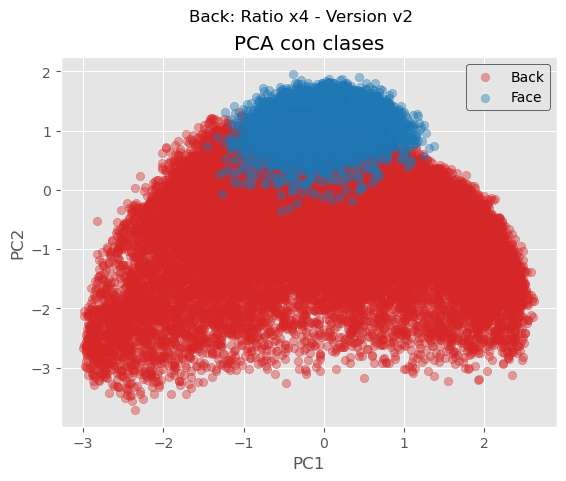
\includegraphics[width=0.6\textwidth]{tarea_1/imagenes/pca_x4_v2.png}
    \caption{Proyección PCA (dos primeras componentes) de los descriptores HOG para rostros y fondos de Places365 con ratio 1 : 4. Se observa el solapamiento de las nubes de clases.}
    \label{fig:pca_ratio4}
\end{figure}

\subsection*{Paradoja «mayor calidad $\neq$ mejor desempeño»}
\begin{itemize}
    \item \textbf{Textura y gradiente}: Los parches de Places365 contienen bordes y contrastes fuertes (edificios, ventanas, mobiliario) que generan firmas HOG parecidas a las facciones faciales —sobre todo a baja escala—.
    \item \textbf{Distribución de frecuencias espaciales}: El \textit{down-scaling} de 256 → 100 px concentra detalle de alta frecuencia en un área reducida, haciendo que muchos parches exhiban patrones verticales u horizontales que la proyección PCA confunde con cejas, nariz u orejas.
    \item \textbf{CIFAR-10 como ruido útil}: Aunque las imágenes de 32 px son de menor fidelidad, sus objetos centrados y fondos difusos aportan gradientes suaves que, paradójicamente, actúan como negativos fáciles: refuerzan la frontera de decisión sin invadir el espacio de los positivos.
\end{itemize}

\subsection*{Síntesis y elección final de dataset}

Los experimentos confirman que la resolución más alta de Places365 no se traduce en un mejor espacio de características para HOG + PCA ni en un incremento de desempeño del clasificador. Por el contrario, los parches de CIFAR-10 —pese a su baja fidelidad— conservan la separación de nubes hasta \textit{ratios} significativamente mayores y sustentan métricas consistentemente superiores. Por esa razón, en las tareas posteriores trabajamos principalmente con el dataset generado a partir de CIFAR-10, incorporando solo un subconjunto depurado de Places365 cuando fue necesario diversificar levemente los negativos. Esta combinación optimiza el balance entre variabilidad útil, costo de filtrado y desempeño global del sistema.


\pagebreak

\section*{Tarea 2: Análisis de Componentes Principales (PCA)}

\subsection*{Metodología}

Los datos del conjunto tienen una dimensionalidad de 4096 features (64×64 = 4096), lo cual representa un espacio de características muy alto. Por esta razón, se aplicó PCA como técnica de reducción de dimensionalidad, para tener un número menor de dimensiones (componentes principales) que mantenga la información más relevante.\\

PCA permite transformar los datos originales en un nuevo espacio de características donde las componentes principales están ordenadas por la cantidad de variabilidad capturada. Esto ayuda a reducir el ruido y la redundancia en los datos, lo que permite acelerar el entrenamiento y mejorar el desempeño de los modelos.\\

Se utilizan las gráficas de varianza explicada y varianza acumulada para visualizar la distribución de la información entre las diferentes componentes principales. La varianza explicada por cada componente principal indica la proporción de información (variabilidad) que representa dicha componente respecto al total. Por su parte, la varianza acumulada muestra cuánta información total se conserva al considerar un cierto número de componentes principales, sumando la varianza explicada de cada una.\\

Para determinar la cantidad adecuada de componentes principales a conservar, se consideraron varios criterios. En primer lugar, se probaron diferentes cantidades de componentes con el objetivo de alcanzar al menos el 95\% de la varianza explicada acumulada, un umbral comúnmente utilizado como guía aunque no es una regla estricta. Otro criterio utilizado fue la observación de la gráfica de varianza acumulada: cuando la curva comienza a formar una meseta, se interpreta que las componentes adicionales aportan poca información que puede ser de utilidad. En base a estos criterios, se evaluaron distintos valores (20, 50, 100, 200, 500 componentes) para identificar el número óptimo que conserve la mayor cantidad posible de información relevante.\\

Por último, se plotean gráficas de dispersión en el espacio de componentes principales para visualizar la distribución de los datos en el nuevo espacio reducido. Estas gráficas permiten observar la separación entre las clases (rostros y fondos) y la efectividad de la reducción de dimensionalidad.\\

Para probar el desempeño de PCA, se implementó un modelo GaussianNB y se lo entrenó con el conjunto de datos de entrenamiento con PCA aplicado. Se utilizó un conjunto de datos balanceado (1:1) y otro desbalanceado (1:2) para comparar los resultados.

\subsection*{Resultados}

% Presentar las componentes principales obtenidas
% Mostrar gráficas de varianza explicada
% Incluir diagramas de dispersión

La primera aplicación de PCA, se hizo sobre un conjunto de datos que incluye mitad rostros y la otra mitad fondos. A continuación se muestran las gráficas de varianza explicada y varianza acumulada para el caso que obtuvo el mejor f1 score sobre el conjunto de validación que fue con 50 componentes principales:\\

\begin{figure}[H]
    \centering
    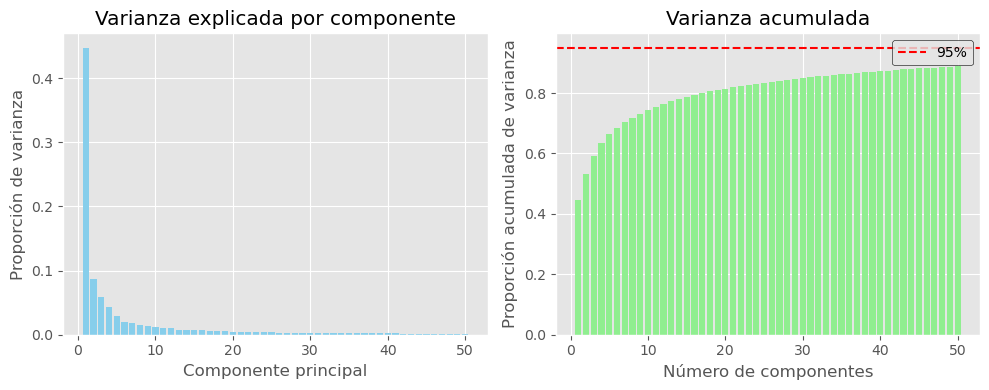
\includegraphics[width=0.8\textwidth]{tarea_2/imagenes/variance_x1_v1_50.png}
    \caption{Varianza explicada y acumulada para 50 componentes (Dataset balanceado 1:1)}
    \label{fig:pca_componentes}
\end{figure}

También se grafican las distribuciones de los datos en el espacio de componentes principales para 2, 3 y 5componentes principales: 

\begin{figure}[H]
    \centering
    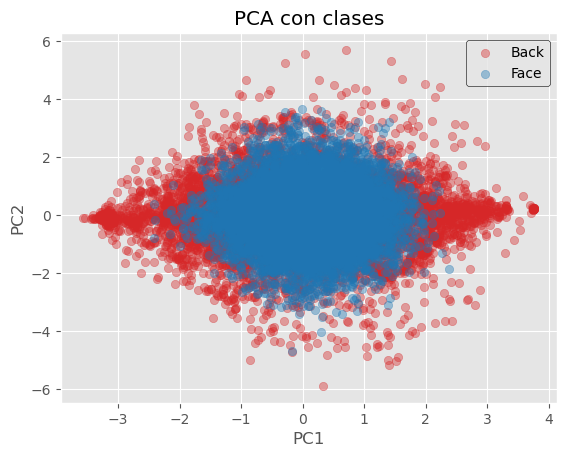
\includegraphics[width=0.7\textwidth]{tarea_2/imagenes/pca_classes_x1_v1_50_2_components.png}
    \caption{Distribución de rostros y fondos en el espacio de componentes principales para 2 componentes principales (Dataset balanceado 1:1)}
    \label{fig:pca_classes}
\end{figure}

\begin{figure}[H]
    \centering
    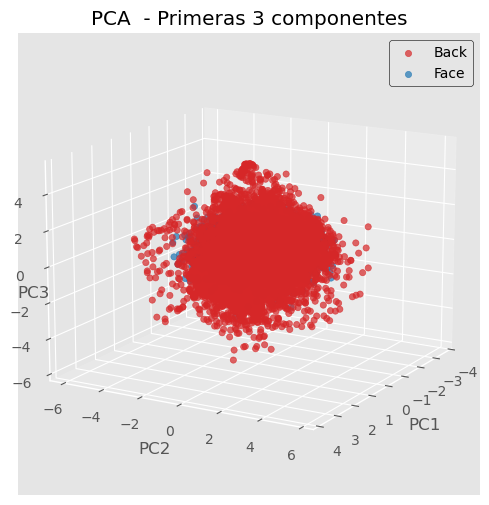
\includegraphics[width=0.7\textwidth]{tarea_2/imagenes/pca_classes_x1_v1_50_3_components.png}
    \caption{Distribución de rostros y fondos en el espacio de componentes principales para 3 componentes principales (Dataset balanceado 1:1)}
    \label{fig:pca_classes}
\end{figure}

\begin{figure}[H]
    \centering
    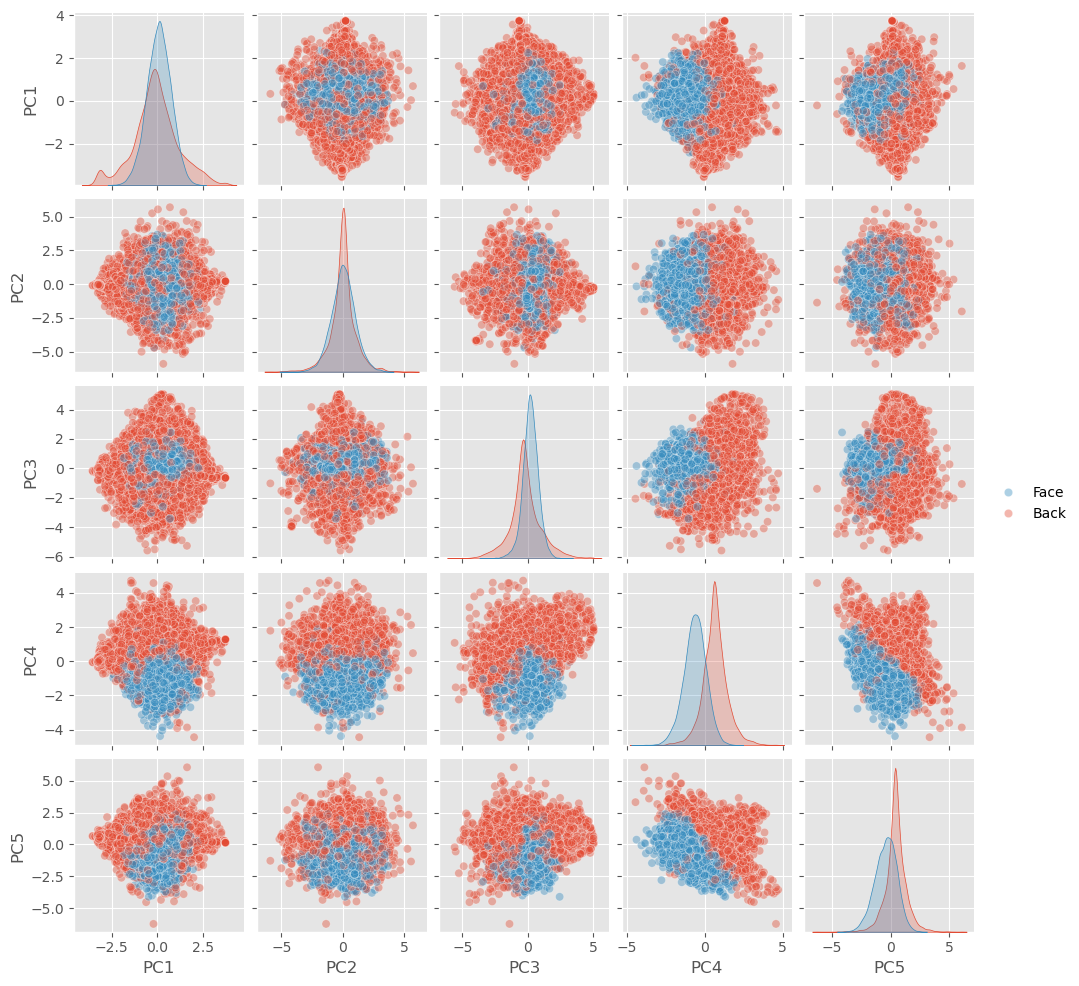
\includegraphics[width=0.8\textwidth]{tarea_2/imagenes/pca_classes_x1_v1_50_5_components.png}
    \caption{Distribución de rostros y fondos en el espacio de componentes principales (5 componentes principales)}
    \label{fig:pca_classes}
\end{figure}

Se registran las métricas obtenidas de los conjuntos de entrenamiento y validación.

\begin{table}[H]
    \centering
    \begin{tabular}{|>{\centering\arraybackslash}m{3.2cm}|c|c|c|c|}
    \hline
    \rowcolor{tableblue} \multicolumn{1}{|c|}{\textbf{Conjunto}} & \textbf{Precisión} & \textbf{Recall} & \textbf{F1-Score} & \textbf{Accuracy} \\
    \hline
    \multicolumn{5}{|c|}{\textbf{Entrenamiento}} \\
    \hline
    Clase 0 (Fondos) & 0.92 & 0.82 & 0.87 & \multirow{2}{*}{0.87} \\
    Clase 1 (Rostros) & 0.84 & 0.93 & 0.88 & \\
    \hline
    \multicolumn{5}{|c|}{\textbf{Validación}} \\
    \hline
    Clase 0 (Fondos) & 0.91 & 0.81 & 0.86 & \multirow{2}{*}{0.87} \\
    Clase 1 (Rostros) & 0.84 & 0.92 & 0.88 & \\
    \hline
    \end{tabular}
    \caption{Métricas de clasificación para 50 componentes principales (Dataset balanceado 1:1)}
    \label{tab:pca_x1_metrics}
\end{table}

Según la \textbf{Figura 2}, las gráficas de varianza explicada y acumulada muestran que, utilizando 50 componentes principales, se alcanza casi el 95\% de la varianza total, lo que justifica la elección de este número de componentes. Además, las \textbf{Figuras 3, 4 y 5} ilustran cómo los datos de rostros y fondos se distribuyen en el espacio de las primeras 2, 3 y 5 componentes principales. Se observa que en todos los casos, las clases presentan una considerable superposición, lo que parecería indicar que las primeras componentes capturan rasgos globales presentes en estas clases.\\

El \textbf{Cuadro 2} muestra las métricas de desempeño. Los valores de \textit{f1-score} son 0.86 para fondos y 0.88 para rostros, lo que indica que el modelo logra un buen equilibrio entre la detección correcta de ambas clases y la minimización de errores de clasificación. La exactitud general (\textit{accuracy}) es de 0.87, reflejando un buen desempeño del modelo en el dataset balanceado. El clasificador tiende a ser más preciso al detectar fondos y más permisivo al detectar rostros (mayor recuperación), lo que sugiere que, aunque el modelo logra distinguir razonablemente bien entre ambas clases, la superposición de características de componentes principales dificulta una separación completamente óptima.\\


% El \textbf{Cuadro 1} resume las métricas de clasificación alcanzadas con 50 componentes principales para el dataset balanceado, donde se logra un \textit{f1-score} de 0.88 para la clase de rostros y 0.87 para fondos en validación, junto a una exactitud global del 87\%.\\

Se aplicó PCA el conjunto de datos que incluye el doble de fondos que de rostros. A continuación se muestran las gráficas de varianza explicada y varianza acumulada para el caso que obtuvo el mejor f1 score sobre el conjunto de validación que fue con 20 componentes principales:

\begin{figure}[H]
    \centering
    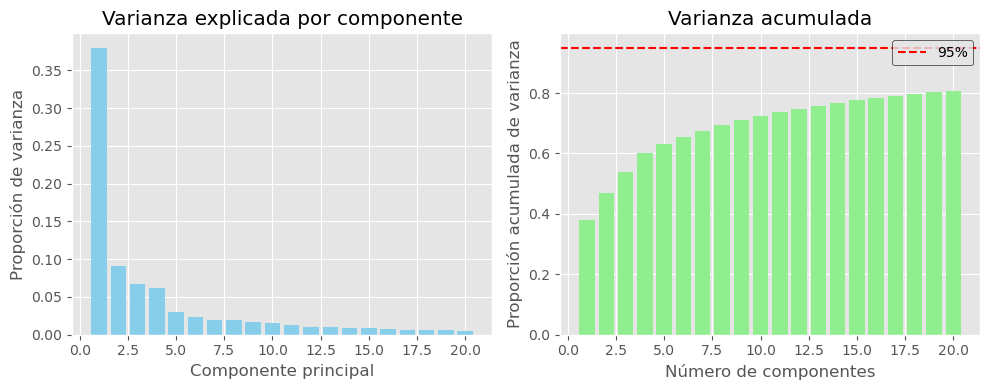
\includegraphics[width=0.8\textwidth]{tarea_2/imagenes/variance_x2_v1_20.png}
    \caption{Varianza explicada y acumulada para 20 componentes (Dataset desbalanceado 1:2)}
    \label{fig:pca_componentes}
\end{figure}

También se grafican las distribuciones de los datos en el espacio de componentes principales para 2, 3 y 5 componentes principales:

\begin{figure}[H]
    \centering
    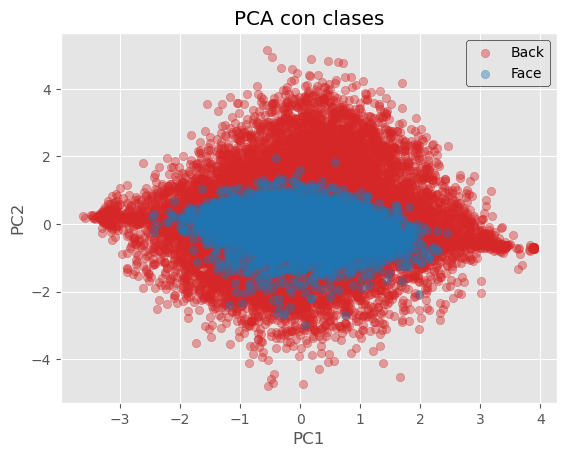
\includegraphics[width=0.7\textwidth]{tarea_2/imagenes/pca_classes_x2_v1_20_2_components.png}
    \caption{Distribución de rostros y fondos en el espacio de componentes principales para 2 componentes principales (Dataset desbalanceado 1:2)}
    \label{fig:pca_classes}
\end{figure}

\begin{figure}[H]
    \centering
    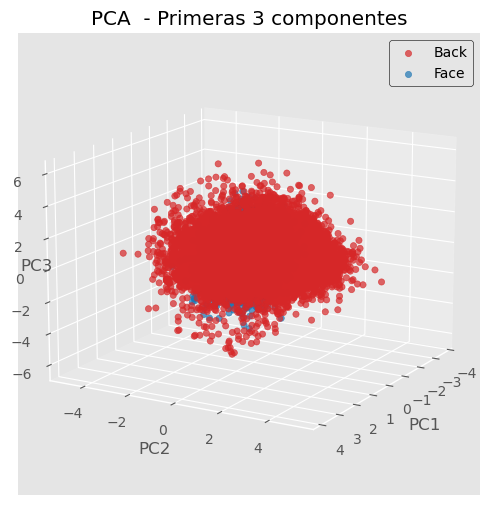
\includegraphics[width=0.7\textwidth]{tarea_2/imagenes/pca_classes_x2_v1_20_3_components.png}
    \caption{Distribución de rostros y fondos en el espacio de componentes principales para 3 componentes principales (Dataset desbalanceado 1:2)}
    \label{fig:pca_classes}
\end{figure}

\begin{figure}[H]
    \centering
    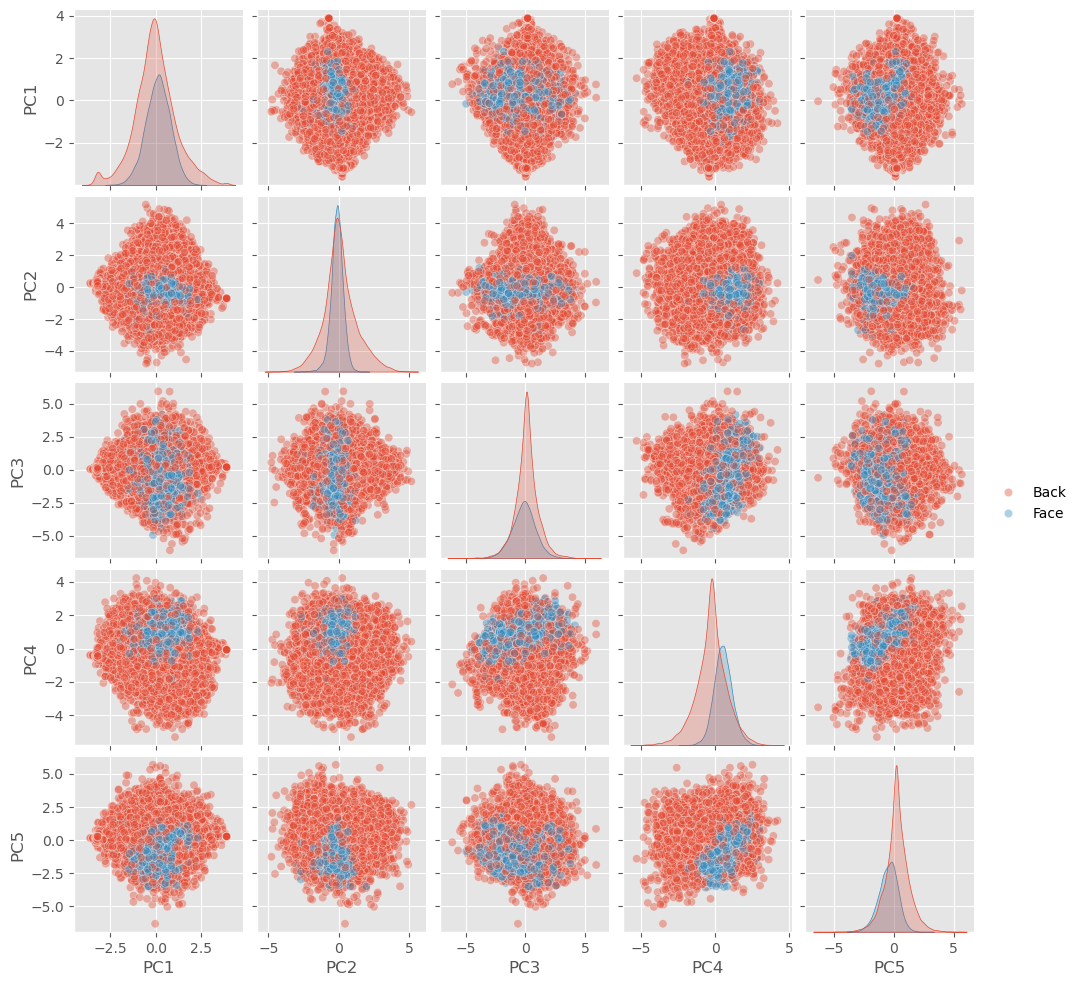
\includegraphics[width=0.8\textwidth]{tarea_2/imagenes/pca_classes_x2_v1_20_5_components.png}
    \caption{Distribución de rostros y fondos en el espacio de componentes principales (5 componentes principales)}
    \label{fig:pca_classes}
\end{figure}

Se registran las métricas obtenidas de los conjuntos de entrenamiento y validación.

\begin{table}[H]
    \centering
    \begin{tabular}{|>{\centering\arraybackslash}m{3.2cm}|c|c|c|c|}
    \hline
    \rowcolor{tableblue} \multicolumn{1}{|c|}{\textbf{Conjunto}} & \textbf{Precisión} & \textbf{Recall} & \textbf{F1-Score} & \textbf{Accuracy} \\
    \hline
    \multicolumn{5}{|c|}{\textbf{Entrenamiento}} \\
    \hline
    Clase 0 (Fondos) & 0.94 & 0.87 & 0.90 & \multirow{2}{*}{0.88} \\
    Clase 1 (Rostros) & 0.77 & 0.89 & 0.83 & \\
    \hline
    \multicolumn{5}{|c|}{\textbf{Validación}} \\
    \hline
    Clase 0 (Fondos) & 0.94 & 0.87 & 0.90 & \multirow{2}{*}{0.88} \\
    Clase 1 (Rostros) & 0.78 & 0.88 & 0.83 & \\
    \hline
    \end{tabular}
    \caption{Métricas de clasificación para 20 componentes principales (Dataset desbalanceado 1:2)}
    \label{tab:pca_x2_metrics}
\end{table}

Según la \textbf{Figura 6}, las gráficas de varianza explicada y acumulada revelan que, al emplear únicamente 20 componentes principales, se preserva una proporción significativa de la varianza total en el conjunto desbalanceado (relación 2:1 de fondos a rostros). Este número de componentes no es el que más se acerca al 95\% de la varianza total, siendo 50 y 100 componentes más próximos a este porcentaje. Sin embargo, es posible que las características que no se capturan favorezcan la generalización del modelo, al evitar que se ajuste demasiado a patrones específicos o ruido del set de entrenamiento. Las \textbf{Figuras 7, 8 y 9} muestran que, al igual que en el caso balanceado, existe una superposición entre las clases en el espacio de componentes principales.\\

El \textbf{Cuadro 3} muestra que los valores de \textit{f1-score} son de 0.90 para fondos y 0.83 para rostros, mientras que la exactitud se eleva a 0.88. Comparando con el escenario balanceado del \textbf{Cuadro 2}, se observa que el modelo incrementa su capacidad para clasificar fondos (mejores puntajes en todas las métricas), pero reduce su capacidad para clasificar rostros (peores puntajes en todas las métricas).\\

Aunque el valor de accuracy aumenta levemente, esto puede ser engañoso, ya que la métrica puede verse influida por la mejora del desempeño sobre la clase predominante. Por lo tanto, se puede concluir que el caso balanceado ofrece un mejor rendimiento para la correcta clasificación de rostros.

\pagebreak
\section*{Tarea 3: Entrega Base}

\subsection*{Metodología}

Para la entrega base, se implementó un clasificador utilizando PCA con 50 componentes principales junto con características HOG. El enfoque adoptado fue:

\begin{enumerate}
    \item \textbf{Dataset}: Se utilizó un dataset balanceado, con igual cantidad de rostros que de fondos.
    \item \textbf{Extracción de características}: Se aplicó HOG a las imágenes de 64×64 píxeles para obtener descriptores de gradientes orientados.
    \item \textbf{Reducción de dimensionalidad}: Se utilizó PCA para reducir a 50 componentes principales, capturando las características más relevantes.
    \item \textbf{Clasificación}: Se entrenó un clasificador usando el modelo GaussianNB sin utilizar StandardScaler, ya que en pruebas iniciales no mejoraba los resultados.
\end{enumerate}

\subsection*{Resultados}

La implementación base logró un puntaje de Kaggle de \textbf{0.97907} (f1 Score).\\

\textbf{Observaciones importantes}:
\begin{itemize}
    \item \textbf{StandardScaler}: Inicialmente no se utilizó porque no mejoraba los resultados. Posteriormente se descubrió que esto se debía a que se estaba aplicando \texttt{fit\_transform} a los datos de validación en lugar de solo \texttt{transform}, lo cual introduce sesgo en la evaluación.
    \item \textbf{Generación de fondos}: Se identificaron problemas en las primeras versiones donde las imágenes de fondo no estaban correctamente escaladas al rango 0-255, afectando la consistencia del preprocesamiento.
\end{itemize}

Estos hallazgos fueron fundamentales para las mejoras implementadas en las tareas posteriores.

\pagebreak

\section*{Tarea 4: Implementación de HOG + PCA}

\subsection*{Metodología}

Se implementó la combinación de HOG (Histogram of Oriented Gradients) con PCA para extraer características más robustas de las imágenes de rostros. A diferencia de la Tarea 2 que aplicaba PCA directamente sobre los píxeles de las imágenes, este enfoque primero extrae descriptores HOG y luego aplica PCA sobre estos descriptores.\\

Para la extracción HOG, se utilizó la función \texttt{skimage.feature.hog} de la biblioteca \texttt{skimage} con los parámetros por defecto pero se decidió experimentar con 2 parámetros para ver si mejoraban los resultados.\\

Los parámetros se ajustaron específicamente son:
\begin{itemize}
    \item \textbf{cells\_per\_block=(2,2)}: Aumenta la granularidad de los descriptores HOG, capturando más detalles locales en las imágenes.
    \item \textbf{transform\_sqrt=True}: Reduce el efecto de variaciones de iluminación y sombras en rostros.
\end{itemize}

Para evaluar el desempeño, se utilizaron las \textbf{mismas condiciones que en la Tarea 2}: mismo clasificador (GaussianNB), mismas cantidades de componentes (20, 50, 100, 200 y 500) y métricas de evaluación. Se probó sobre el conjunto balanceado (1:1) y el desbalanceado (1:2) con los parámetros por defecto de la función \texttt{hog} y con los cambios propuestos.

\subsection*{Resultados}

\textbf{Conjunto balanceado (1:1) - HOG + PCA}:\\

Se encontró que 20 componentes proporcionó el mejor resultado en el conjunto de validación. A continuación se muestran las gráficas de varianza explicada y varianza acumulada para este caso:

\begin{figure}[H]
    \centering
    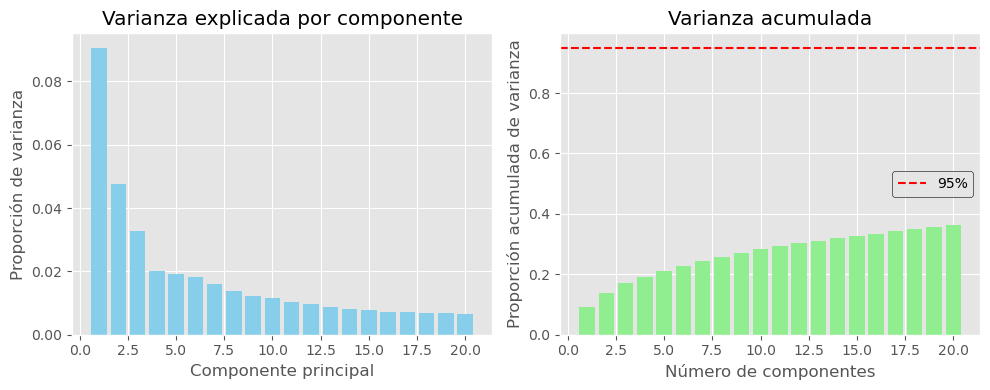
\includegraphics[width=0.8\textwidth]{tarea_4/imagenes/variance_x1_v1_20.png}
    \caption{Varianza explicada y acumulada para 20 componentes HOG + PCA (Dataset balanceado 1:1)}
    \label{fig:hog_pca_variance_x1}
\end{figure}

También se grafican las distribuciones de los datos en el espacio de componentes principales para 2, 3 y 5 componentes principales:

\begin{figure}[H]
    \centering
    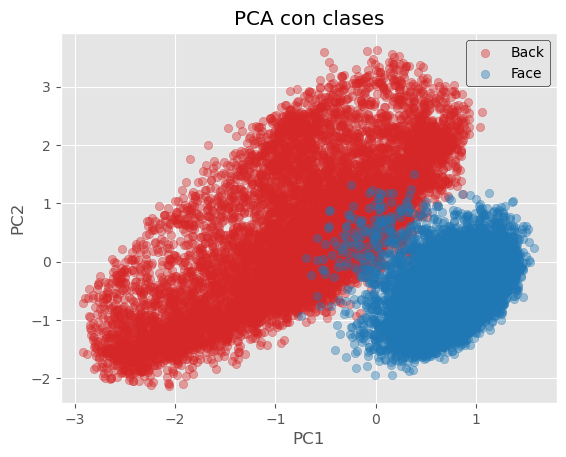
\includegraphics[width=0.6\textwidth]{tarea_4/imagenes/pca_classes_x1_v1_20_2_components.png}
    \caption{Distribución de rostros y fondos en el espacio de componentes principales para 2 componentes principales PCA+HOG (Dataset balanceado 1:1)}
    \label{fig:pca_classes}
\end{figure}

\begin{figure}[H]
    \centering
    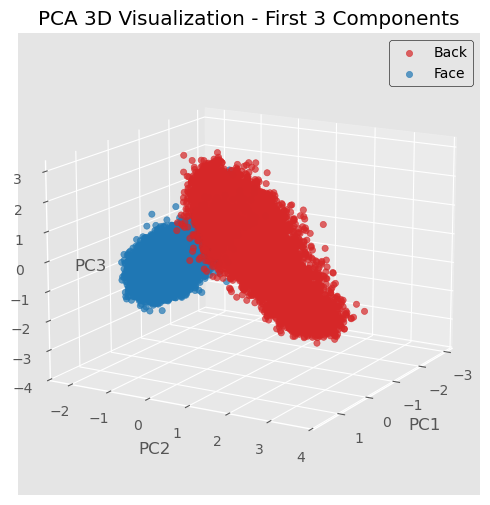
\includegraphics[width=0.6\textwidth]{tarea_4/imagenes/pca_classes_x1_v1_20_3_components.png}
    \caption{Distribución de rostros y fondos en el espacio de componentes principales para 3 componentes principales PCA+HOG (Dataset balanceado 1:1)}
    \label{fig:pca_classes}
\end{figure}

\begin{figure}[H]
    \centering
    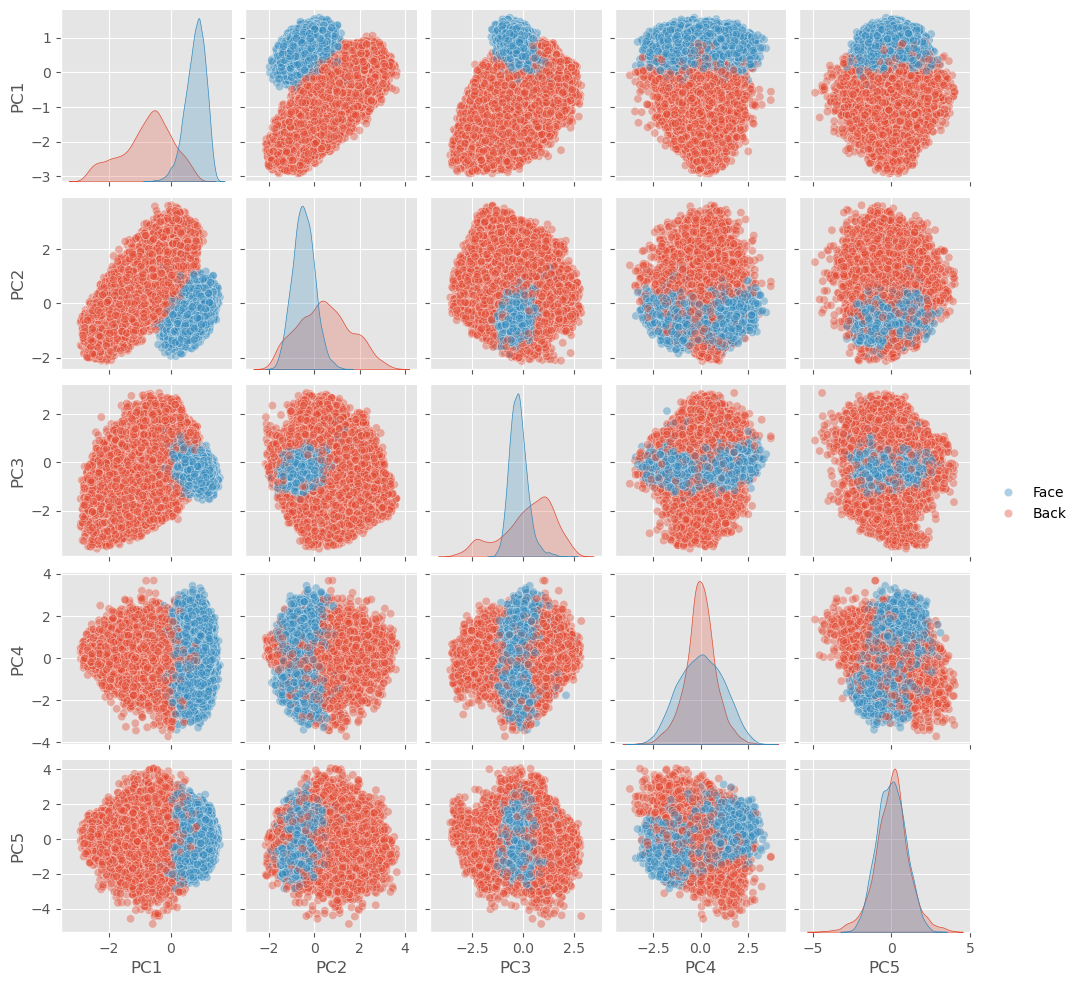
\includegraphics[width=0.8\textwidth]{tarea_4/imagenes/pairplot_x1_v1_20.png}
    \caption{Distribución de rostros y fondos en el espacio de componentes principales (5 componentes principales)}
    \label{fig:pca_classes}
\end{figure}

Se registran las métricas obtenidas de los conjuntos de entrenamiento y validación.

\begin{table}[H]
    \centering
    \begin{tabular}{|>{\centering\arraybackslash}m{3.2cm}|c|c|c|c|}
    \hline
    \rowcolor{tableblue} \multicolumn{1}{|c|}{\textbf{Conjunto}} & \textbf{Precisión} & \textbf{Recall} & \textbf{F1-Score} & \textbf{Accuracy} \\
    \hline
    \multicolumn{5}{|c|}{\textbf{Entrenamiento}} \\
    \hline
    Clase 0 (Fondos) & 0.97 & 1.00 & 0.98 & \multirow{2}{*}{0.98} \\
    Clase 1 (Rostros) & 1.00 & 0.96 & 0.98 & \\
    \hline
    \multicolumn{5}{|c|}{\textbf{Validación}} \\
    \hline
    Clase 0 (Fondos) & 0.97 & 1.00 & 0.98 & \multirow{2}{*}{0.98} \\
    Clase 1 (Rostros) & 1.00 & 0.97 & 0.98 & \\
    \hline
    \end{tabular}
    \caption{Métricas de clasificación para 100 componentes HOG + PCA (Dataset balanceado 1:1)}
    \label{tab:hog_pca_x1_metrics}
\end{table}

\textbf{Conjunto balanceado (1:1) - HOG (con modificaciones) + PCA}:\\

Se encontró que 20 componentes proporcionó el mejor resultado en el conjunto de validación. A continuación se muestran las gráficas de varianza explicada y varianza acumulada para este caso:

\begin{figure}[H]
    \centering
    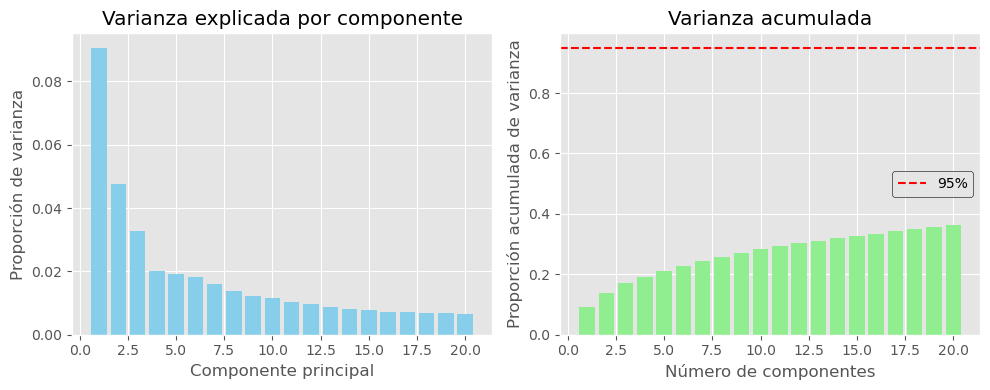
\includegraphics[width=0.8\textwidth]{tarea_4/imagenes/variance_x1_v1_20.png}
    \caption{Varianza explicada y acumulada para 20 componentes HOG + PCA (Dataset balanceado 1:1)}
    \label{fig:hog_pca_variance_x1}
\end{figure}

También se grafican las distribuciones de los datos en el espacio de componentes principales para 2, 3 y 5 componentes principales:

\begin{figure}[H]
    \centering
    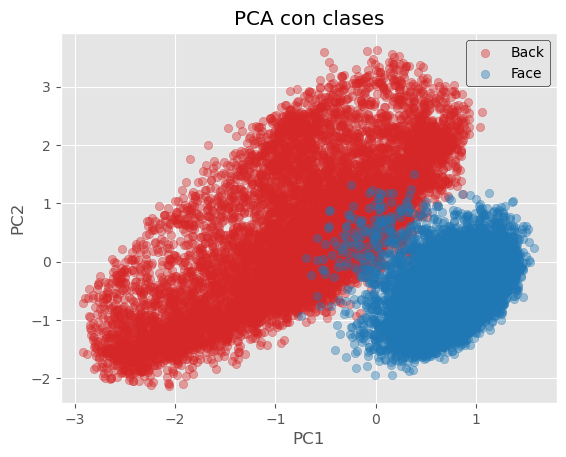
\includegraphics[width=0.6\textwidth]{tarea_4/imagenes/pca_classes_x1_v1_20_2_components.png}
    \caption{Distribución de rostros y fondos en el espacio de componentes principales para 2 componentes principales PCA+HOG (Dataset balanceado 1:1)}
    \label{fig:pca_classes}
\end{figure}

\begin{figure}[H]
    \centering
    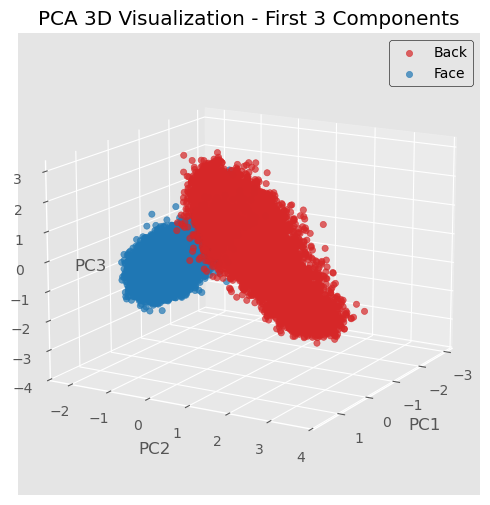
\includegraphics[width=0.6\textwidth]{tarea_4/imagenes/pca_classes_x1_v1_20_3_components.png}
    \caption{Distribución de rostros y fondos en el espacio de componentes principales para 3 componentes principales PCA+HOG (Dataset balanceado 1:1)}
    \label{fig:pca_classes}
\end{figure}

\begin{figure}[H]
    \centering
    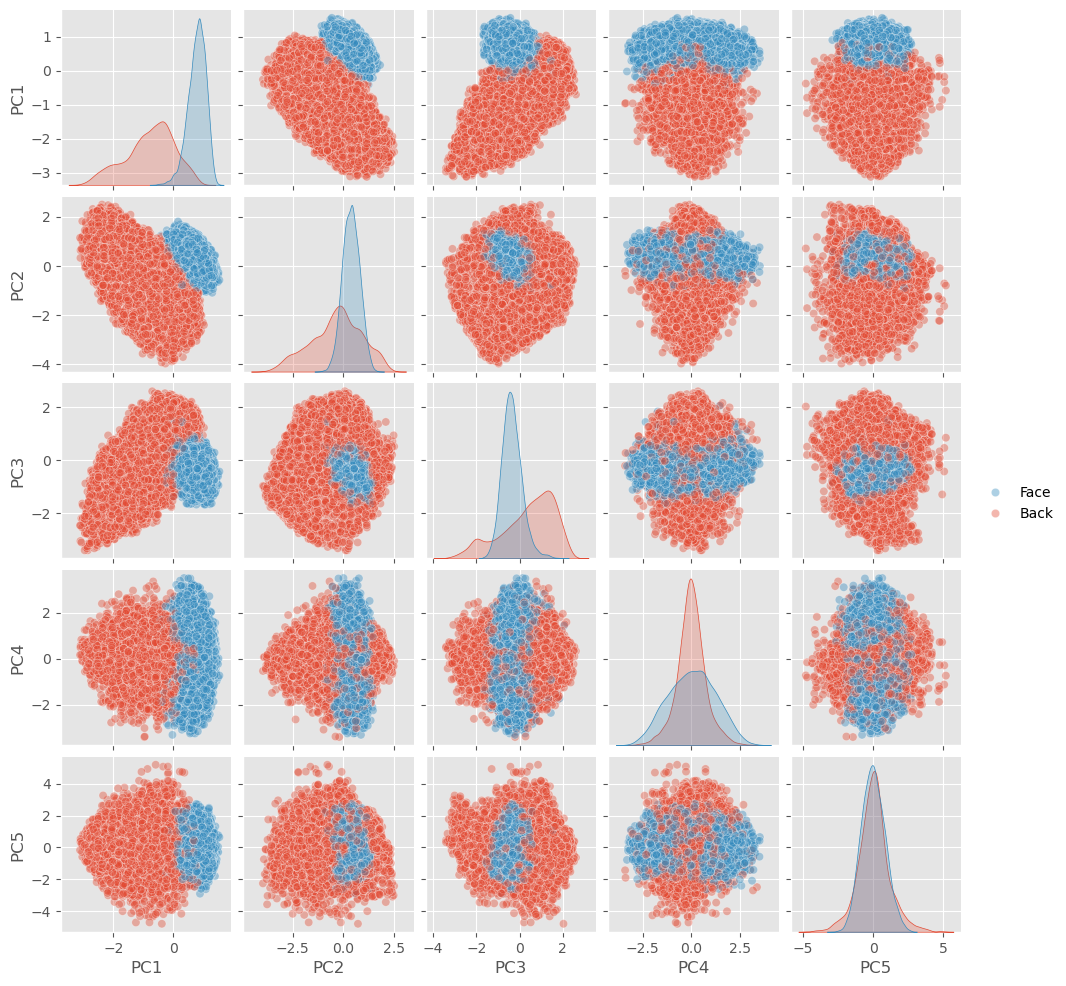
\includegraphics[width=0.8\textwidth]{tarea_4/imagenes/pairplot_cambios_hog_x1_v1_20.png}
    \caption{Distribución de rostros y fondos en el espacio de componentes principales (5 componentes principales)}
    \label{fig:pca_classes}
\end{figure}

Se registran las métricas obtenidas de los conjuntos de entrenamiento y validación.

\begin{table}[H]
    \centering
    \begin{tabular}{|>{\centering\arraybackslash}m{3.2cm}|c|c|c|c|}
    \hline
    \rowcolor{tableblue} \multicolumn{1}{|c|}{\textbf{Conjunto}} & \textbf{Precisión} & \textbf{Recall} & \textbf{F1-Score} & \textbf{Accuracy} \\
    \hline
    \multicolumn{5}{|c|}{\textbf{Entrenamiento}} \\
    \hline
    Clase 0 (Fondos) & 0.97 & 1.00 & 0.98 & \multirow{2}{*}{0.98} \\
    Clase 1 (Rostros) & 1.00 & 0.96 & 0.98 & \\
    \hline
    \multicolumn{5}{|c|}{\textbf{Validación}} \\
    \hline
    Clase 0 (Fondos) & 0.97 & 1.00 & 0.98 & \multirow{2}{*}{0.98} \\
    Clase 1 (Rostros) & 1.00 & 0.97 & 0.98 & \\
    \hline
    \end{tabular}
    \caption{Métricas de clasificación para 100 componentes HOG (con modificaciones) + PCA (Dataset balanceado 1:1)}
    \label{tab:hog_pca_x1_metrics}
\end{table}

\textbf{Conjunto desbalanceado (1:2) - HOG + PCA}:\\

Se encontró que 20 componentes proporcionó el mejor resultado en el conjunto de validación. A continuación se muestran las gráficas de varianza explicada y varianza acumulada para este caso:
\begin{figure}[H]
    \centering
    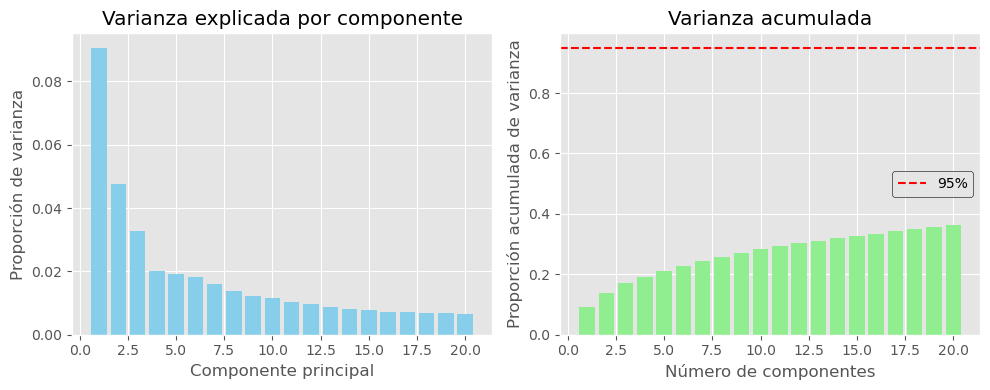
\includegraphics[width=0.8\textwidth]{tarea_4/imagenes/variance_x1_v1_20.png}
    \caption{Varianza explicada y acumulada para 20 componentes HOG + PCA (Dataset desbalanceado 1:2)}
    \label{fig:hog_pca_variance_x1}
\end{figure}

También se grafican las distribuciones de los datos en el espacio de componentes principales para 2, 3 y 5 componentes principales:

\begin{figure}[H]
    \centering
    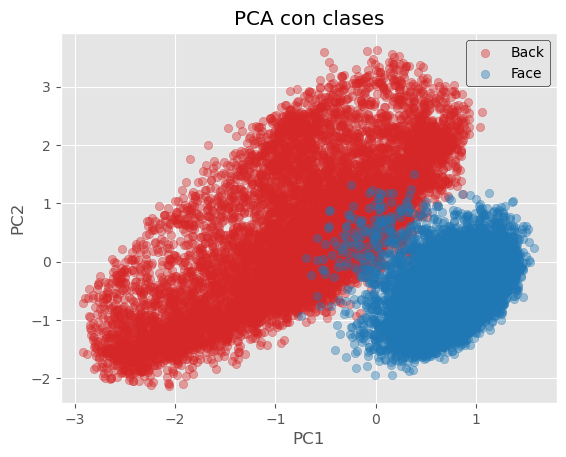
\includegraphics[width=0.6\textwidth]{tarea_4/imagenes/pca_classes_x1_v1_20_2_components.png}
    \caption{Distribución de rostros y fondos en el espacio de componentes principales para 2 componentes principales PCA+HOG (Dataset balanceado 1:1)}
    \label{fig:pca_classes}
\end{figure}

\begin{figure}[H]
    \centering
    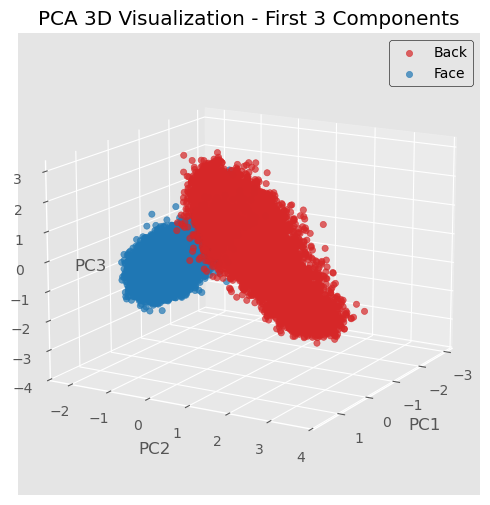
\includegraphics[width=0.6\textwidth]{tarea_4/imagenes/pca_classes_x1_v1_20_3_components.png}
    \caption{Distribución de rostros y fondos en el espacio de componentes principales para 3 componentes principales PCA+HOG (Dataset balanceado 1:2)}
    \label{fig:pca_classes}
\end{figure}

\begin{figure}[H]
    \centering
    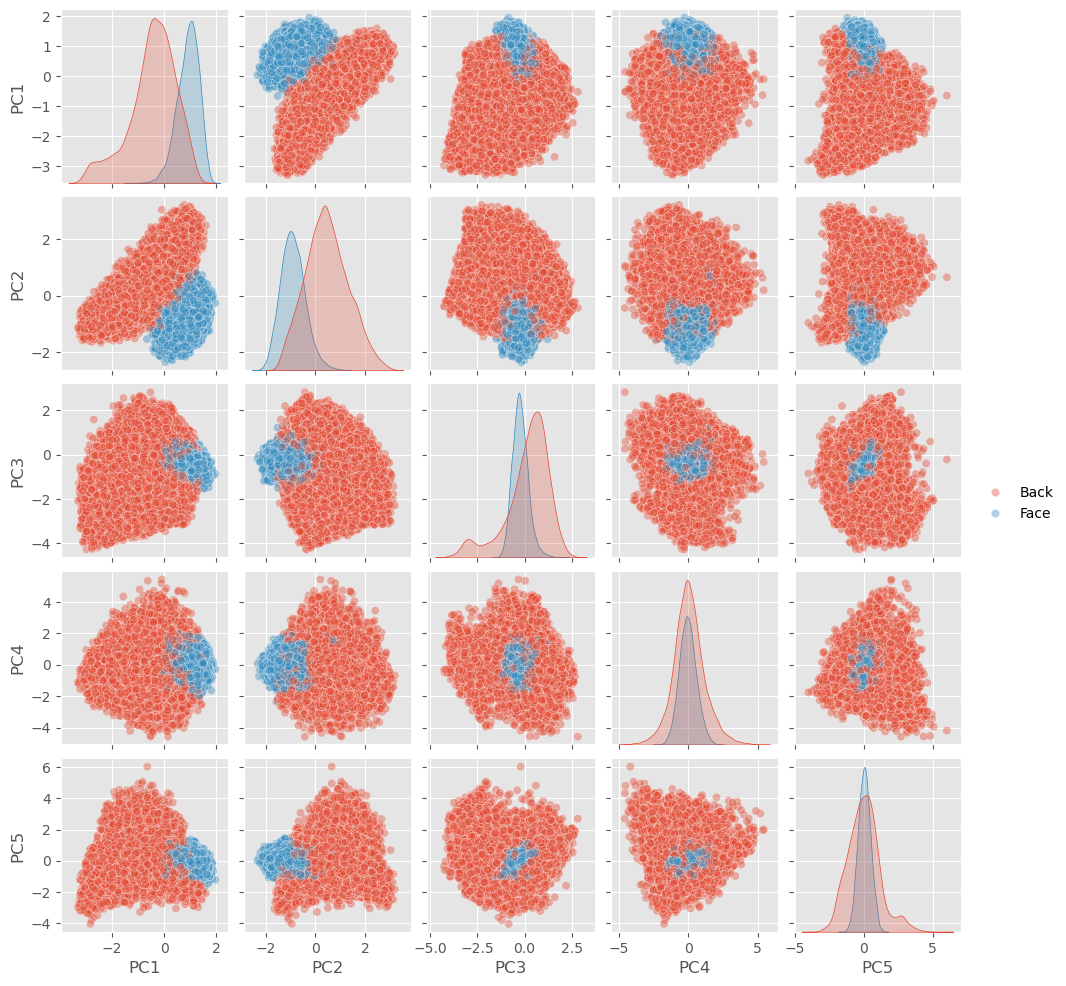
\includegraphics[width=0.8\textwidth]{tarea_4/imagenes/pairplot_x2_v1_20.png}
    \caption{Distribución de rostros y fondos en el espacio de componentes principales (5 componentes principales)}
    \label{fig:pca_classes}
\end{figure}

Se registran las métricas obtenidas de los conjuntos de entrenamiento y validación.

\begin{table}[H]
    \centering
    \begin{tabular}{|>{\centering\arraybackslash}m{3.2cm}|c|c|c|c|}
    \hline
    \rowcolor{tableblue} \multicolumn{1}{|c|}{\textbf{Conjunto}} & \textbf{Precisión} & \textbf{Recall} & \textbf{F1-Score} & \textbf{Accuracy} \\
    \hline
    \multicolumn{5}{|c|}{\textbf{Entrenamiento}} \\
    \hline
    Clase 0 (Fondos) & 0.98 & 1.00 & 0.99 & \multirow{2}{*}{0.98} \\
    Clase 1 (Rostros) & 1.00 & 0.95 & 0.97 & \\
    \hline
    \multicolumn{5}{|c|}{\textbf{Validación}} \\
    \hline
    Clase 0 (Fondos) & 0.98 & 1.00 & 0.99 & \multirow{2}{*}{0.99} \\
    Clase 1 (Rostros) & 1.00 & 0.96 & 0.98 & \\
    \hline
    \end{tabular}
    \caption{Métricas de clasificación para 100 componentes HOG + PCA (Dataset desbalanceado 1:2)}
    \label{tab:hog_pca_x1_metrics}
\end{table}

\textbf{Conjunto desbalanceado (1:2) - HOG (con modificaciones) + PCA}:\\

Se encontró que 20 componentes proporcionó el mejor resultado en el conjunto de validación. A continuación se muestran las gráficas de varianza explicada y varianza acumulada para este caso:

\begin{figure}[H]
    \centering
    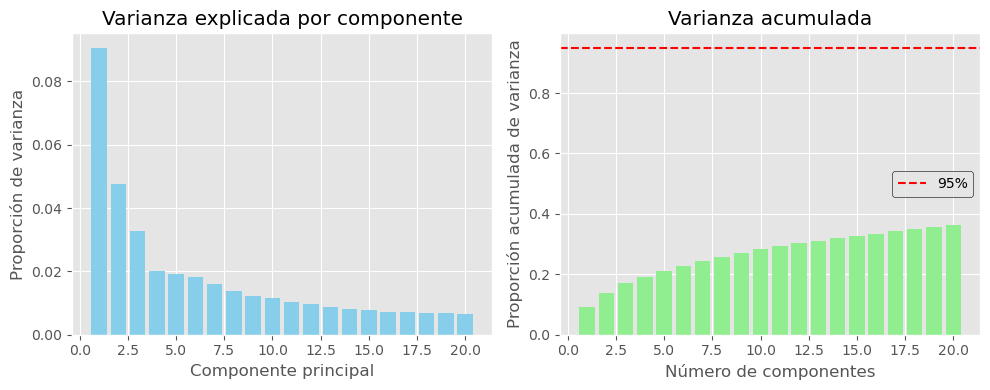
\includegraphics[width=0.8\textwidth]{tarea_4/imagenes/variance_x1_v1_20.png}
    \caption{Varianza explicada y acumulada para 20 componentes HOG + PCA (Dataset balanceado 1:2)}
    \label{fig:hog_pca_variance_x1}
\end{figure}

También se grafican las distribuciones de los datos en el espacio de componentes principales para 2, 3 y 5 componentes principales:

\begin{figure}[H]
    \centering
    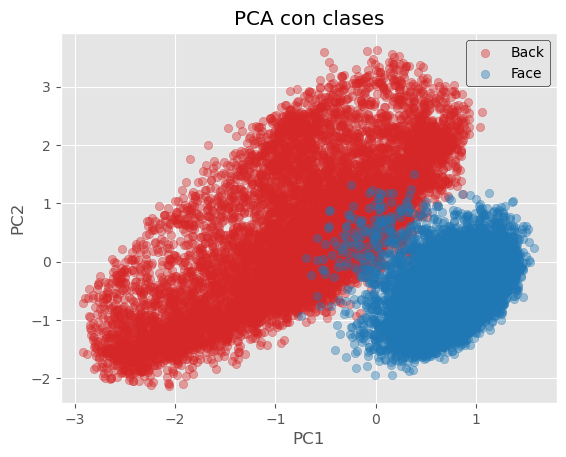
\includegraphics[width=0.6\textwidth]{tarea_4/imagenes/pca_classes_x1_v1_20_2_components.png}
    \caption{Distribución de rostros y fondos en el espacio de componentes principales para 2 componentes principales PCA+HOG (Dataset balanceado 1:1)}
    \label{fig:pca_classes}
\end{figure}

\begin{figure}[H]
    \centering
    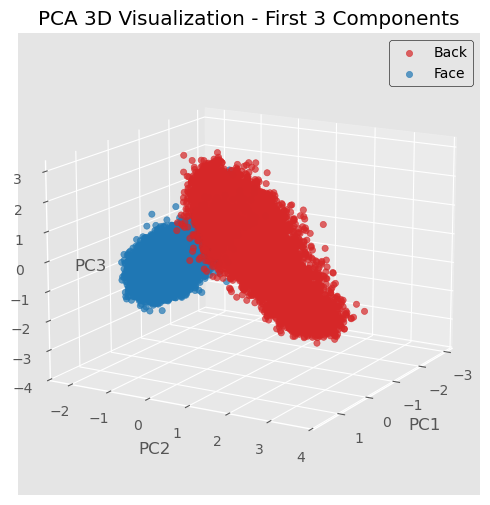
\includegraphics[width=0.6\textwidth]{tarea_4/imagenes/pca_classes_x1_v1_20_3_components.png}
    \caption{Distribución de rostros y fondos en el espacio de componentes principales para 3 componentes principales PCA+HOG (Dataset balanceado 1:2)}
    \label{fig:pca_classes}
\end{figure}

\begin{figure}[H]
    \centering
    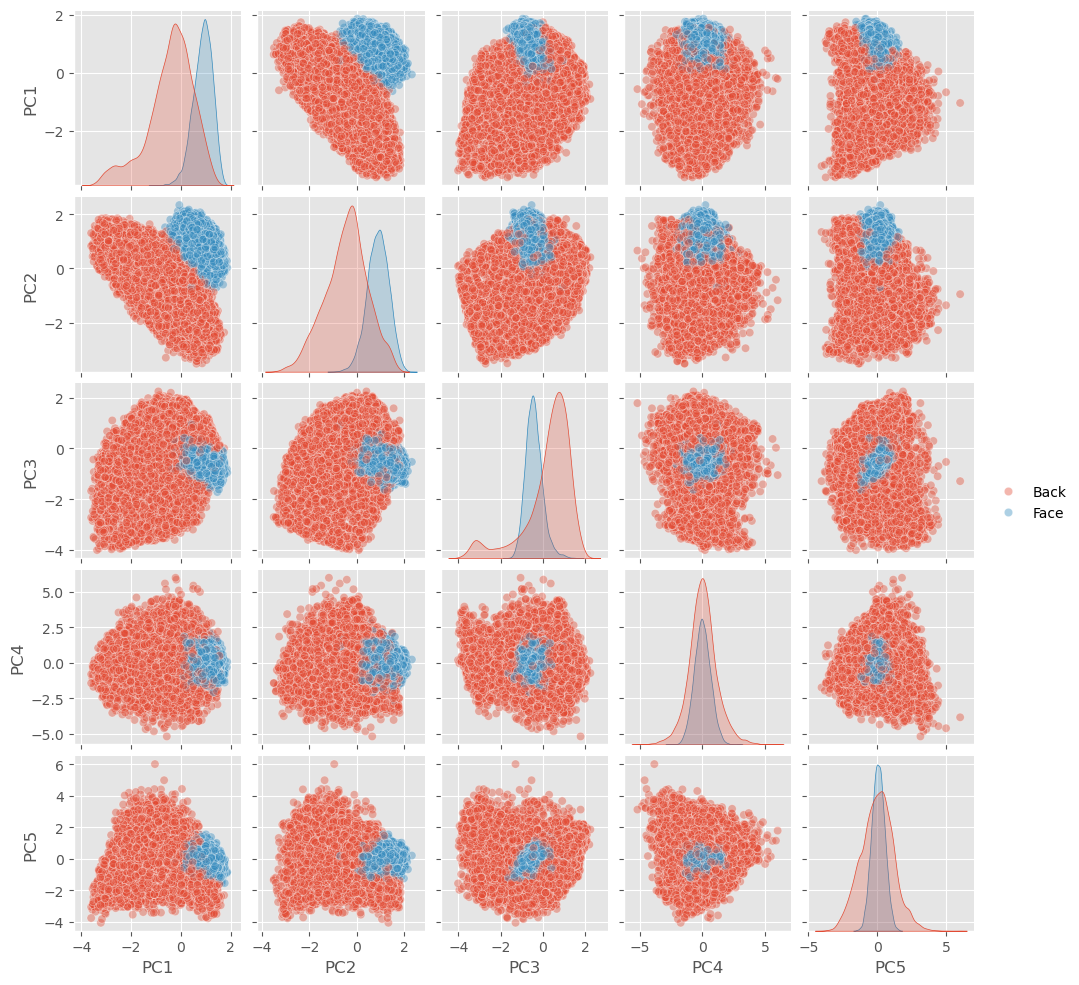
\includegraphics[width=0.8\textwidth]{tarea_4/imagenes/pairplot_cambios_hog_x2_v1_20.png}
    \caption{Distribución de rostros y fondos en el espacio de componentes principales (5 componentes principales)}
    \label{fig:pca_classes}
\end{figure}

Se registran las métricas obtenidas de los conjuntos de entrenamiento y validación.

\begin{table}[H]
    \centering
    \begin{tabular}{|>{\centering\arraybackslash}m{3.2cm}|c|c|c|c|}
    \hline
    \rowcolor{tableblue} \multicolumn{1}{|c|}{\textbf{Conjunto}} & \textbf{Precisión} & \textbf{Recall} & \textbf{F1-Score} & \textbf{Accuracy} \\
    \hline
    \multicolumn{5}{|c|}{\textbf{Entrenamiento}} \\
    \hline
    Clase 0 (Fondos) & 0.98 & 1.00 & 0.99 & \multirow{2}{*}{0.98} \\
    Clase 1 (Rostros) & 1.00 & 0.96 & 0.98 & \\
    \hline
    \multicolumn{5}{|c|}{\textbf{Validación}} \\
    \hline
    Clase 0 (Fondos) & 0.98 & 1.00 & 0.99 & \multirow{2}{*}{0.99} \\
    Clase 1 (Rostros) & 1.00 & 0.96 & 0.98 & \\
    \hline
    \end{tabular}
    \caption{Métricas de clasificación para 100 componentes HOG (con modificaciones) + PCA (Dataset balanceado 1:2)}
    \label{tab:hog_pca_x1_metrics}
\end{table}

\textbf{Comparación HOG + PCA vs PCA (mismo clasificador y condiciones)}:\\

Se seleccionaron los mejores casos de PCA solo y HOG + PCA para las métricas de validación en clasificación de rostros y se compararon:

\begin{table}[H]
    \centering
    \begin{tabular}{|>{\centering\arraybackslash}m{2.7cm}|>{\centering\arraybackslash}m{3.2cm}|c|c|c|c|c|}
    \hline
    \rowcolor{tableblue} \multicolumn{1}{|c|}{\textbf{Método}} & \multicolumn{1}{c|}{\textbf{Dataset}} & \textbf{Componentes} & \textbf{Precisión} & \textbf{Recall} & \textbf{F1-Score} & \textbf{Accuracy} \\
    \hline
    PCA solo & Balanceado (1:1) & 50 & 0.84 & 0.92 & 0.88 & 0.87 \\
    HOG + PCA & Balanceado (1:1) & 20 & \textbf{1.00} & \textbf{0.97} & \textbf{0.98} & \textbf{0.98} \\
    \hline
    PCA solo & Desbalanceado (1:2) & 20 & 0.78 & 0.88 & 0.83 & 0.88 \\
    HOG (con cambios) + PCA & Desbalanceado (1:2) & 20 & \textbf{1.00} & \textbf{0.96} & \textbf{0.98} & \textbf{0.99} \\
    \hline
    \end{tabular}
    \caption{Comparación directa entre PCA y HOG + PCA usando GaussianNB - Métricas de rostros}
    \label{tab:comparison_pca_hog_faces}
\end{table}

Las gráficas de dispersión HOG + PCA muestran una \textbf{mejor separación entre clases} comparado con PCA solo, especialmente en las primeras dos componentes principales. Esto se debe a que HOG extrae características locales basadas en la orientación de los gradientes, lo que las hace más discriminativas para distinguir rostros de fondos, mientras que PCA aplicado directamente a píxeles captura principalmente variaciones globales de intensidad.\\

Los resultados de la tabla demuestran mejoras importantes de HOG + PCA sobre PCA solo en ambos escenarios:

\begin{itemize}
    \item \textbf{Conjunto balanceado (1:1)}: HOG + PCA con 20 componentes supera significativamente a PCA solo con 50 componentes, logrando una precisión máxima (1.00) versus 0.84, y mejoras de 10 puntos en F1-Score (0.98 vs 0.88) y 9 en accuracy (0.98 vs 0.87).

    \item \textbf{Conjunto desbalanceado (1:2)}: HOG + PCA con 20 componentes mantiene una precisión máxima (1.00) comparado con 0.78 de PCA solo, con mejoras de 15 puntos en F1-Score (0.98 vs 0.83) y 11 puntos en accuracy (0.99 vs 0.88).
\end{itemize}

HOG + PCA logra mejores resultados utilizando menos componentes (20 vs 50 para el caso balanceado), demostrando que las características HOG son más informativas y requieren menor dimensionalidad para capturar patrones relevantes.\\

Los parámetros optimizados (\texttt{cells\_per\_block=(2,2)} y \texttt{transform\_sqrt=True}) contribuyeron a tener mejores resultados al capturar mejor los detalles de los rostros con bloques más pequeños y reducir los efectos de variaciones de iluminación. Esto se dio para las cantidades de componentes 20, 50, 100 y 200. Para 500 componentes, los parámetros por defecto de \texttt{hog} tuvieron un mejor desempeño.\\

La combinación HOG + PCA demuestra ser superior a utilizar solo PCA, estableciendo una base sólida para los experimentos con múltiples clasificadores en la Tarea 5.

\pagebreak

\section*{Tarea 5: Evaluación de Modelos}

\subsection*{Metodología}

Se implementaron y evaluaron diferentes modelos y técnicas de selección vistas en clase, para la clasificación de imágenes utilizando diferentes estrategias de cross-validation y búsqueda de hiperparámetros. Una vez obtenidos los mejores hiperparámetros, se entrenaron los modelos finales con el conjunto completo de entrenamiento. Se ordenaron según su mejor puntaje de Kaggle y sobre los tres mejores modelos, se amplió la búsqueda en conjuntos de imágenes mayores y se registraron las métricas evaluadas.

\subsubsection*{Proceso de evaluación detallado}

\textbf{Experimentación inicial}:\\

El proceso de evaluación tuvo una etapa previa de experimentación en la que se entrenaron varios modelos con una cantidad de componentes de PCA fija (50) que fue la utilizada para la entrega base. El dataset es balanceado, es un conjunto de imágenes donde hay una cantidad similar de rostros (12833) y fondos (12800). Se utilizó una estrategia de GridSearch para encontrar los mejores hiperparámetros de cada modelo combinado con ShuffleSplit como técnica de cross-validation por recomendación del profesor en una clase de la materia. Luego se hizo un submit a Kaggle de las predicciones de cada modelo (entrenado solo con el set de training) para ver que tan bien se desempeñaban con datos no vistos.\\

La información obtenida a partir de esto se utilizó para descartar algunos modelos que tuvieron los desempeños más bajos y para tener una base de hiperparámetros para el proceso más formal de evaluación.\\

\textbf{Metodología de evaluación}:\\

El proceso de evaluación se realizó en las siguientes etapas:

\begin{enumerate}
    \item Entrenar un dataset desbalanceado (12833 rostros y 25600 fondos) con todos los modelos elegidos con 20, 50, 100, 150, 200, 500 componentes de PCA + HOG, utilizando diferentes estrategias de exploración de hiperparámetros y cross-validation. Para las cantidades de componentes 20, 50, 100 y 200 se utilizaron los parámetros de HOG modificados (cells\_per\_block=(2,2) y transform\_sqrt=True) que habían demostrado ser efectivos en la Tarea 4. Para 500 componentes se utilizaron los parámetros por defecto de HOG.
    \item Elegir el mejor resultado para cada modelo (mejor cantidad de componentes e hiperparámetros) y entrenar con todo el dataset para cada modelo.
    \item Hacer el submit a Kaggle para ver puntaje de cada modelo entrenado con el dataset completo y seleccionar el que presenta mejores resultados en varias métricas de evaluación.
    % \item Generar conjuntos de fondos x5, x10, x20.
    % \item Elegir los mejores 3 modelos, entrenarlos con 20, 50, 100, 150, 200 y 500 componentes y usar GridSearch para encontrar los mejores hiperparámetros.
    % \item Comparar con todas las métricas para elegir el mejor resultado entre todos los modelos y entrenarlo con todo el dataset.
    % \item Hacer nuevamente el submit a Kaggle con el modelo final.
\end{enumerate}
\subsection*{Clasificadores}

\textbf{Redes Neuronales}:
\begin{itemize}
    \item MLPClassifier
\end{itemize}

\textbf{Métodos de Ensemble}:
\begin{itemize}
    \item AdaBoostClassifier, GradientBoostingClassifier, XGBClassifier, BaggingClassifier, RandomForestClassifier
\end{itemize}

\textbf{Modelos Lineales}:
\begin{itemize}
    \item LogisticRegression
\end{itemize}

\textbf{Modelos Probabilísticos}:
\begin{itemize}
    \item GaussianNB
\end{itemize}

\textbf{Modelos Basados en Instancias}:
\begin{itemize}
    \item KNeighborsClassifier
\end{itemize}

\textbf{Modelos Basados en Árboles}:
\begin{itemize}
    \item DecisionTreeClassifier
\end{itemize}

\subsection*{Evaluación y selección de modelos}

\textbf{Métodos de validación y búsqueda de hiperparámetros}:
\begin{itemize}
    \item \textbf{Búsqueda de hiperparámetros}: Se compararon diferentes enfoques:
    \begin{itemize}
        \item \textbf{GridSearchCV}: Búsqueda exhaustiva que evalúa todas las combinaciones posibles de hiperparámetros en un espacio de búsqueda definido.
        \item \textbf{RandomizedSearchCV con 100 iteraciones}: Búsqueda aleatoria que muestrea un número fijo de combinaciones de hiperparámetros del espacio de búsqueda.
    \end{itemize}
    \item \textbf{Cross-Validation}: Se evaluaron múltiples estrategias:
    \begin{itemize}
        \item \textbf{ShuffleSplit con 5 divisiones, 20\% para prueba}: Divide aleatoriamente los datos en conjuntos de entrenamiento y prueba múltiples veces. No garantiza que todas las muestras sean usadas para validación, pero introduce alta variabilidad entre divisiones.
        \item \textbf{StratifiedKFold con 5 divisiones y shuffle}: Divide los datos en K pliegues manteniendo la proporción de clases en cada pliegue. Garantiza que cada muestra sea usada exactamente una vez para validación, proporcionando estimaciones más estables.
        \item \textbf{StratifiedShuffleSplit con 5 divisiones, 20\% para prueba}: Combina la estratificación (preservación de proporciones de clases) con la aleatoriedad de ShuffleSplit.
    \end{itemize}
    \item \textbf{Combinaciones evaluadas}: GridSearch + ShuffleSplit, RandomizedSearch + StratifiedKFold, GridSearch + StratifiedShuffleSplit, GridSearch + StratifiedKFold
    \item \textbf{Métrica de selección de mejores hiperparámetros}: F1-score
\end{itemize}

\textbf{Métricas de clasificación básicas}:

Se registran las siguientes métricas de clasificación para los modelos evaluados (para la clase de rostros):

\begin{itemize}
    \item \textbf{Precision (precisión por clase)}: Proporción de verdaderos positivos sobre el total de predicciones positivas (TP/(TP+FP)). Mide qué tan confiables son las predicciones positivas del modelo.
    \item \textbf{Recall (sensibilidad o tasa de verdaderos positivos)}: Proporción de verdaderos positivos sobre el total de casos positivos reales (TP/(TP+FN)). Mide qué tan bien el modelo identifica todos los casos positivos.
    \item \textbf{F1-Score (métrica principal de evaluación)}: Media armónica entre precisión y recall. Proporciona un balance entre ambas métricas, siendo especialmente útil cuando las clases están desbalanceadas.
    \item \textbf{Accuracy (precisión general del modelo)}: Proporción de predicciones correctas sobre el total de predicciones.
\end{itemize}

\textbf{Métricas de evaluación ROC}:
\begin{itemize}
    \item \textbf{AUC-ROC (área bajo la curva ROC)}: Mide la capacidad del modelo para distinguir entre clases a través de todos los umbrales de clasificación.
    \item \textbf{TPR (True Positive Rate - tasa de verdaderos positivos)}: Equivalente a recall, mide la proporción de casos positivos correctamente identificados. TPR = TP/(TP+FN).
    \item \textbf{FPR (False Positive Rate - tasa de falsos positivos)}: Proporción de casos negativos incorrectamente clasificados como positivos. FPR = FP/(FP+TN). Un FPR bajo significa que el modelo comete pocos errores al clasificar imágenes de fondos como rostros (falsos positivos).
    \item \textbf{G-Mean (media geométrica entre TPR y TNR)}: Raíz cuadrada del producto entre TPR y TNR (True Negative Rate). Proporciona un balance entre la sensibilidad y especificidad, siendo útil para datasets desbalanceados.
\end{itemize}

\textbf{Evaluación externa y análisis visual}:
\begin{itemize}
    \item \textbf{F1-Score (resultado de competencia de Kaggle)}: Evaluación independiente en datos completamente no vistos, proporcionando una medida objetiva del rendimiento de generalización del modelo en condiciones reales.
    \item \textbf{Análisis de curvas ROC y matrices de confusión}: Herramientas visuales para evaluar el rendimiento del modelo. Las curvas ROC muestran el trade-off entre TPR y FPR, mientras que las matrices de confusión revelan patrones específicos de errores de clasificación.
\end{itemize}

\textbf{Hiperparámetros explorados}:
\begin{itemize}
    \item \textbf{MLPClassifier} \\max\_iter [1000, 1500, 2000], solver [adam], learning\_rate\_init [0.0001, 0.001, 0.01], hidden\_layer\_sizes [(50,), (100,), (50, 50), (60, 120, 15)], alpha [0.0001, 0.001], activation [relu]
    \item \textbf{AdaBoost} \\estimator\_\_max\_depth [1, 2], n\_estimators [50, 100, 200], learning\_rate [0.1, 0.5, 1.0]
    \item \textbf{GradientBoosting} \\n\_estimators [100, 200], learning\_rate [0.05, 0.1], max\_depth [None, 1, 3, 5]
    \item \textbf{XGBoost} \\n\_estimators [30, 50, 100, 200, 300], learning\_rate [0.001, 0.05, 0.1, 0.2], max\_depth [None, 1, 3, 5, 10]
    \item \textbf{DecisionTree} \\max\_depth [None, 10, 20, 30], min\_samples\_split [2, 5, 10]
    \item \textbf{Bagging} \\estimator\_\_max\_depth [None, 10, 20], n\_estimators [20, 50, 100]
    \item \textbf{RandomForest} \\n\_estimators [100, 200], max\_depth [None, 5, 10, 20], min\_samples\_split [2, 5, 10]
    \item \textbf{KNeighbors} \\n\_neighbors [3, 5, 7, 10, 15], weights [uniform, distance]
    \item \textbf{LogisticRegression} \\C [0.1, 1, 10, 100], solver [liblinear, lbfgs]
    \item \textbf{GaussianNB} \\Sin hiperparámetros
\end{itemize}

\subsection*{Resultados}

\textbf{Tablas comparativas de resultados de la experimentación inicial}:

\begin{table}[H]
    \centering
    \begin{tabular}{|l|l|c|c|}
    \hline
    \rowcolor{tableblue} \textbf{Modelo} & \textbf{Mejores Hiperparámetros} & \textbf{F1-Score (CV)} & \textbf{Kaggle F1-Score} \\
    \hline
    \textbf{MLPClassifier} & \begin{tabular}[c]{@{}l@{}}activation='relu', alpha=0.0001,\\ hidden\_layer\_sizes=(100,),\\ learning\_rate\_init=0.01, max\_iter=1000,\\ solver='adam'\end{tabular} & 0.9973 & \textbf{0.99173} \\
    \hline
    \textbf{RandomForest} & max\_depth=20, n\_estimators=200 & 0.9913 & 0.98755 \\
    \hline
    \textbf{XGBoost} & max\_depth=3, n\_estimators=200 & 0.9957 & 0.98755 \\
    \hline
    \textbf{GradientBoosting} & max\_depth=5, n\_estimators=200 & 0.9941 & 0.97142 \\
    \hline
    \textbf{GaussianNB} & - & 0.9797 & 0.96638 \\
    \hline
    \textbf{Bagging} & n\_estimators=100 & 0.9912 & 0.95582 \\
    \hline
    \textbf{LogisticRegression} & C=1.0, penalty='l2' & 0.9924 & 0.94117 \\
    \hline
    \textbf{DecisionTree} & max\_depth=10 & 0.9861 & 0.87407 \\
    \hline
    \textbf{AdaBoost} & n\_estimators=50 & 0.9853 & 0.80546 \\
    \hline
    \textbf{KNeighbors} & n\_neighbors=3 & 0.9760 & 0.76190 \\
    \hline
    \end{tabular}
    \caption{Hiperparámetros óptimos, F1-Score de cross-validation y resultados de Kaggle}
    \label{tab:hiperparametros}
\end{table}

\textbf{Desempeño de los modelos}:\\

Los tres mejores modelos según resultados de Kaggle fueron:
\begin{enumerate}
    \item \textbf{MLPClassifier}: F1=0.9973 (CV), Kaggle=0.99173
    \item \textbf{RandomForest}: F1=0.9913 (CV), Kaggle=0.98755
    \item \textbf{XGBoost}: F1=0.9957 (CV), Kaggle=0.98755
\end{enumerate}

El \textbf{MLPClassifier} mantuvo su liderazgo tanto en validación como en Kaggle. RandomForest y XGBoost obtuvieron el mismo puntaje en Kaggle (0.98755), aunque XGBoost tuvo mejor F1-Score en validación. En contrapartida, k-NN mostró el menor desempeño (Kaggle=0.76190).\\

A raíz de estos resultados, se decidió no continuar con la evaluación de DecisionTree, Bagging y KNeighbors. Los criterios utilizados fueron bajo desempeño (KNeighbors y DecisionTree) y priorizar RandomForest sobre Bagging porque RandomForest es una técnica de ensamblado más robusta y generalmente ofrece mejor rendimiento como se demuestra en el resultado de Kaggle.\\

\textbf{Evaluación final}:\\

Durante el desarrollo de la metodología de evaluación, se experimentó con diferentes combinaciones de técnicas de validación cruzada y búsqueda de hiperparámetros para optimizar el rendimiento de los modelos:

\begin{enumerate}
    \item \textbf{GridSearch + ShuffleSplit}: Búsqueda exhaustiva con división aleatoria de datos

\begin{table}[H]
    \centering
    \begin{tabular}{|l|c|c|c|c|c|p{4cm}|}
    \hline
    \rowcolor{tableblue} \textbf{Modelo} & \textbf{PCA} & \textbf{Accuracy} & \textbf{Precision} & \textbf{Recall} & \textbf{F1-Score} & \textbf{Hiperparámetros} \\
    \hline
    \textbf{MLPClassifier} & 200 & 0.9975 & 0.9996 & 0.9930 & 0.9963 & \small{activation=relu, alpha=0.001, hidden\_layer\_sizes=(100,), learning\_rate\_init=0.01, max\_iter=1000, solver=adam} \\
    \hline
    \textbf{AdaBoost} & 100 & 0.9966 & 0.9984 & 0.9915 & 0.9949 & \small{estimator\_\_max\_depth=2, learning\_rate=1.0, n\_estimators=200} \\
    \hline
    \textbf{XGBoost} & 100 & 0.9964 & 0.9981 & 0.9911 & 0.9946 & \small{learning\_rate=0.2, max\_depth=3, n\_estimators=300} \\
    \hline
    \textbf{LogisticRegression} & 200 & 0.9955 & 0.9969 & 0.9895 & 0.9932 & \small{C=0.1, solver=lbfgs} \\
    \hline
    \textbf{GradientBoosting} & 50 & 0.9948 & 0.9973 & 0.9872 & 0.9922 & \small{learning\_rate=0.1, max\_depth=5, n\_estimators=200} \\
    \hline
    \textbf{RandomForest} & 20 & 0.9935 & 0.9992 & 0.9814 & 0.9902 & \small{max\_depth=20, min\_samples\_split=2, n\_estimators=200} \\
    \hline
    \textbf{GaussianNB} & 20 & 0.9874 & 0.9988 & 0.9636 & 0.9809 & \small{Sin hiperparámetros} \\
    \hline
    \end{tabular}
    \caption{Métricas de clasificación principales - GridSearch + ShuffleSplit}
    \label{tab:metricas_gridsearch_shufflesplit}
\end{table}

    \item \textbf{RandomizedSearch + StratifiedKFold}: Búsqueda aleatoria con división estratificada en K pliegues

\begin{table}[H]
    \centering
    \begin{tabular}{|l|c|c|c|c|c|p{4cm}|}
    \hline
    \rowcolor{tableblue} \textbf{Modelo} & \textbf{PCA} & \textbf{Accuracy} & \textbf{Precision} & \textbf{Recall} & \textbf{F1-Score} & \textbf{Hiperparámetros} \\
    \hline
    \textbf{MLPClassifier} & 100 & 0.9979 & 0.9992 & 0.9946 & 0.9969 & \small{activation=relu, alpha=0.001, hidden\_layer\_sizes=(100,), learning\_rate\_init=0.01, max\_iter=1000, solver=adam} \\
    \hline
    \textbf{XGBoost} & 100 & 0.9974 & 0.9996 & 0.9926 & 0.9961 & \small{learning\_rate=0.2, max\_depth=3, n\_estimators=300} \\
    \hline
    \textbf{AdaBoost} & 50 & 0.9962 & 0.9984 & 0.9903 & 0.9944 & \small{estimator\_\_max\_depth=2, learning\_rate=1.0, n\_estimators=200} \\
    \hline
    \textbf{GradientBoosting} & 50 & 0.9952 & 0.9965 & 0.9892 & 0.9928 & \small{learning\_rate=0.1, max\_depth=5, n\_estimators=200} \\
    \hline
    \textbf{LogisticRegression} & 200 & 0.9944 & 0.9953 & 0.9880 & 0.9916 & \small{C=0.1, solver=liblinear} \\
    \hline
    \textbf{RandomForest} & 20 & 0.9939 & 0.9996 & 0.9822 & 0.9908 & \small{max\_depth=None, min\_samples\_split=5, n\_estimators=200} \\
    \hline
    \textbf{GaussianNB} & 20 & 0.9857 & 0.9984 & 0.9590 & 0.9783 & \small{Sin hiperparámetros} \\
    \hline
    \end{tabular}
    \caption{Métricas de clasificación principales - RandomizedSearch + StratifiedKFold}
    \label{tab:metricas_randomizedsearch_stratifiedkfold}
\end{table}

    \item \textbf{GridSearch + StratifiedShuffleSplit}: Búsqueda exhaustiva con división estratificada aleatoria

\begin{table}[H]
    \centering
    \begin{tabular}{|l|c|c|c|c|c|p{4cm}|}
    \hline
    \rowcolor{tableblue} \textbf{Modelo} & \textbf{PCA} & \textbf{Accuracy} & \textbf{Precision} & \textbf{Recall} & \textbf{F1-Score} & \textbf{Hiperparámetros} \\
    \hline
    \textbf{MLPClassifier} & 200 & 0.9981 & 0.9996 & 0.9946 & 0.9971 & \small{activation=relu, alpha=0.0001, hidden\_layer\_sizes=(100,), learning\_rate\_init=0.01, max\_iter=1000, solver=adam} \\
    \hline
    \textbf{AdaBoost} & 100 & 0.9968 & 0.9973 & 0.9930 & 0.9952 & \small{estimator\_\_max\_depth=2, learning\_rate=1.0, n\_estimators=200} \\
    \hline
    \textbf{XGBoost} & 500 & 0.9964 & 0.9988 & 0.9903 & 0.9946 & \small{learning\_rate=0.2, max\_depth=3, n\_estimators=300} \\
    \hline
    \textbf{LogisticRegression} & 200 & 0.9953 & 0.9965 & 0.9895 & 0.9930 & \small{C=0.1, solver=liblinear} \\
    \hline
    \textbf{GradientBoosting} & 500 & 0.9951 & 0.9969 & 0.9884 & 0.9926 & \small{learning\_rate=0.1, max\_depth=5, n\_estimators=200} \\
    \hline
    \textbf{RandomForest} & 20 & 0.9931 & 0.9992 & 0.9803 & 0.9896 & \small{max\_depth=None, min\_samples\_split=2, n\_estimators=200} \\
    \hline
    \textbf{GaussianNB} & 20 & 0.9868 & 0.9992 & 0.9613 & 0.9799 & \small{Sin hiperparámetros} \\
    \hline
    \end{tabular}
    \caption{Métricas de clasificación principales - GridSearch + StratifiedShuffleSplit}
    \label{tab:metricas_gridsearch_stratifiedshufflesplit}
\end{table}

    \item \textbf{GridSearch + StratifiedKFold}: Búsqueda exhaustiva con división estratificada en K pliegues.

\begin{table}[H]
    \centering
    \begin{tabular}{|l|c|c|c|c|c|p{4cm}|}
    \hline
    \rowcolor{tableblue} \textbf{Modelo} & \textbf{PCA} & \textbf{Accuracy} & \textbf{Precision} & \textbf{Recall} & \textbf{F1-Score} & \textbf{Hiperparámetros} \\
    \hline
    \textbf{MLPClassifier} & 200 & 0.9978 & 0.9988 & 0.9946 & 0.9967 & \small{activation=relu, alpha=0.0001, hidden\_layer\_sizes=(100,), learning\_rate\_init=0.01, max\_iter=1000, solver=adam} \\
    \hline
    \textbf{XGBoost} & 50 & 0.9962 & 0.9973 & 0.9915 & 0.9944 & \small{learning\_rate=0.2, max\_depth=3, n\_estimators=300} \\
    \hline
    \textbf{AdaBoost} & 100 & 0.9961 & 0.9980 & 0.9903 & 0.9942 & \small{estimator\_\_max\_depth=2, learning\_rate=1.0, n\_estimators=200} \\
    \hline
    \textbf{LogisticRegression} & 200 & 0.9956 & 0.9969 & 0.9899 & 0.9934 & \small{C=0.1, solver=liblinear} \\
    \hline
    \textbf{GradientBoosting} & 50 & 0.9951 & 0.9973 & 0.9880 & 0.9926 & \small{learning\_rate=0.1, max\_depth=3, n\_estimators=200} \\
    \hline
    \textbf{RandomForest} & 20 & 0.9935 & 0.9992 & 0.9814 & 0.9902 & \small{max\_depth=None, min\_samples\_split=2, n\_estimators=200} \\
    \hline
    \textbf{GaussianNB} & 20 & 0.9861 & 0.9988 & 0.9597 & 0.9789 & \small{Sin hiperparámetros} \\
    \hline
    \end{tabular}
    \caption{Métricas de clasificación principales - GridSearch + StratifiedKFold}
    \label{tab:metricas_gridsearch_stratifiedkfold}
\end{table}
\end{enumerate}

\textbf{Mejor resultado global (por modelo)}:

\begin{table}[H]
    \centering
    \begin{tabular}{|l|c|c|c|c|c|c|}
    \hline
    \rowcolor{tableblue} \textbf{Modelo} & \textbf{PCA} & \textbf{Accuracy} & \textbf{Precision} & \textbf{Recall} & \textbf{F1-Score} & \textbf{Kaggle F1-Score} \\
    \hline
    \textbf{MLPClassifier} & 200 & 0.9981 & 0.9996 & 0.9946 & 0.9971 & 1.00000 \\
    \hline
    \textbf{XGBoost} & 100 & 0.9974 & 0.9996 & 0.9926 & 0.9961 & 0.99581 \\
    \hline
    \textbf{AdaBoost} & 100 & 0.9968 & 0.9973 & 0.9930 & 0.9952 & 0.98333 \\
    \hline
    \textbf{LogisticRegression} & 200 & 0.9956 & 0.9969 & 0.9899 & 0.9934 & 0.93385 \\
    \hline
    \textbf{GradientBoosting} & 50 & 0.9952 & 0.9965 & 0.9892 & 0.9928 & 0.98755 \\
    \hline
    \textbf{RandomForest} & 20 & 0.9939 & 0.9996 & 0.9822 & 0.9908 & 0.99166 \\
    \hline
    \textbf{GaussianNB} & 20 & 0.9874 & 0.9988 & 0.9636 & 0.9809 & 0.97890 \\
    \hline
    \end{tabular}
    \caption{Métricas de clasificación principales - Mejores resultados globales}
    \label{tab:metricas_globales}
\end{table}

\begin{table}[H]
    \centering
    \begin{tabular}{|l|l|p{4cm}|}
    \hline
    \rowcolor{tableblue} \textbf{Modelo} & \textbf{Estrategia} & \textbf{Hiperparámetros} \\
    \hline
    \textbf{MLPClassifier} & GridSearch + StratifiedShuffleSplit & \small{activation=relu, alpha=0.0001, hidden\_layer\_sizes=(100,), learning\_rate\_init=0.01, max\_iter=1000, solver=adam} \\
    \hline
    \textbf{XGBoost} & RandomizedSearch + StratifiedKFold & \small{learning\_rate=0.2, max\_depth=3, n\_estimators=300} \\
    \hline
    \textbf{AdaBoost} & GridSearch + StratifiedShuffleSplit & \small{estimator\_\_max\_depth=2, learning\_rate=1.0, n\_estimators=200} \\
    \hline
    \textbf{LogisticRegression} & GridSearch + StratifiedKFold & \small{C=0.1, solver=liblinear} \\
    \hline
    \textbf{GradientBoosting} & RandomizedSearch + StratifiedKFold & \small{learning\_rate=0.1, max\_depth=5, n\_estimators=200} \\
    \hline
    \textbf{RandomForest} & RandomizedSearch + StratifiedKFold & \small{max\_depth=None, min\_samples\_split=5, n\_estimators=200} \\
    \hline
    \textbf{GaussianNB} & GridSearch + ShuffleSplit & \small{Sin hiperparámetros} \\
    \hline
    \end{tabular}%
    \caption{Estrategias e hiperparámetros - Mejores resultados globales}
    \label{tab:estrategias_globales}
\end{table}

% \begin{table}[H]
%     \centering
%     \begin{tabular}{|l|c|c|c|c|}
%     \hline
%     \rowcolor{tableblue} \textbf{Modelo} & \textbf{TPR} & \textbf{FPR} & \textbf{AUC-ROC} & \textbf{G-Mean} \\
%     \hline
%     \textbf{MLPClassifier} & 0.9946 & 0.0002 & 0.9999 & 0.9972 \\
%     \hline
%     \textbf{XGBoost} & 0.9926 & 0.0002 & 0.9997 & 0.9962 \\
%     \hline
%     \textbf{AdaBoost} & 0.9930 & 0.0014 & 0.9995 & 0.9958 \\
%     \hline
%     \textbf{LogisticRegression} & 0.9899 & 0.0016 & 0.9995 & 0.9942 \\
%     \hline
%     \textbf{GradientBoosting} & 0.9892 & 0.0018 & 0.9993 & 0.9937 \\
%     \hline
%     \textbf{RandomForest} & 0.9822 & 0.0002 & 0.9988 & 0.9910 \\
%     \hline
%     \textbf{GaussianNB} & 0.9636 & 0.0006 & 0.9983 & 0.9813 \\
%     \hline
%     \end{tabular}%
%     \caption{Métricas de evaluación ROC y G-Mean - Mejores resultados globales}
%     \label{tab:metricas_roc_globales}
% \end{table}

\textbf{Mejor resultado global}:

\begin{table}[H]
    \centering
    \begin{tabular}{|c|l|c|c|c|c|c|c|}
    \hline
    \rowcolor{tableblue} \textbf{Rank} & \textbf{Modelo} & \textbf{PCA} & \textbf{Accuracy} & \textbf{Precision} & \textbf{Recall} & \textbf{F1-Score} & \textbf{Kaggle F1-Score} \\
    \hline
    % \rowcolor{purple!30} 1 & \textbf{MLPClassifier} & 200 & 0.9981 & 0.9996 & 0.9946 & 0.9971 \\
    \rowcolor{purple!30} 1 & \textbf{MLPClassifier} & 200 & 0.9981 & 0.9996 & 0.9946 & 0.9971 & 1.00000 \\
    \hline
    \rowcolor{blue!20} 2 & \textbf{MLPClassifier} & 100 & 0.9979 & 0.9992 & 0.9946 & 0.9969 & 0.99585 \\
    \hline
    \rowcolor{purple!30} 3 & \textbf{MLPClassifier} & 200 & 0.9978 & 0.9988 & 0.9946 & 0.9967 & 0.99585 \\
    \hline
    \rowcolor{purple!30} 4 & \textbf{MLPClassifier} & 200 & 0.9975 & 0.9996 & 0.9930 & 0.9963 & 0.99173 \\
    \hline
    \rowcolor{purple!30} 5 & \textbf{MLPClassifier} & 200 & 0.9975 & 0.9984 & 0.9942 & 0.9963 & 0.98765 \\
    \hline
    \rowcolor{green!20} 6 & \textbf{MLPClassifier} & 500 & 0.9974 & 0.9988 & 0.9934 & 0.9961 & 0.99585 \\
    \hline
    \rowcolor{yellow!60} 7 & \textbf{XGBoost} & 100 & 0.9974 & 0.9996 & 0.9926 & 0.9961 & 0.98581 \\
    \hline
    \rowcolor{blue!20} 8 & \textbf{MLPClassifier} & 100 & 0.9973 & 0.9992 & 0.9926 & 0.9959 & 0.98347 \\
    \hline
    \rowcolor{green!20} 9 & \textbf{MLPClassifier} & 500 & 0.9973 & 0.9992 & 0.9926 & 0.9959 & 0.98744 \\
    \hline
    \rowcolor{orange!40} 10 & \textbf{MLPClassifier} & 50 & 0.9971 & 0.9984 & 0.9930 & 0.9957 & 0.99166 \\
    \hline
    \end{tabular}
    \caption{Top 10 resultados globales entre todas las estrategias y modelos (Ordenado por F1-Score)}
    \label{tab:top10_globales}
\end{table}

\begin{table}[H]
    \centering
    \begin{tabular}{|c|l|l|p{3.5cm}|}
    \hline
    \rowcolor{tableblue} \textbf{Rank} & \textbf{Modelo} & \textbf{Estrategia} & \textbf{Hiperparámetros} \\
    \hline
    \rowcolor{purple!30} 1 & \textbf{MLPClassifier} & GridSearch + StratifiedShuffleSplit & \tiny{activation=relu, alpha=0.0001, hidden\_layer\_sizes=(100,), learning\_rate\_init=0.01, max\_iter=1000, solver=adam} \\
    \hline
    \rowcolor{blue!20} 2 & \textbf{MLPClassifier} & RandomizedSearch + StratifiedKFold & \tiny{activation=relu, alpha=0.001, hidden\_layer\_sizes=(100,), learning\_rate\_init=0.01, max\_iter=1000, solver=adam} \\
    \hline
    \rowcolor{purple!30} 3 & \textbf{MLPClassifier} & GridSearch + StratifiedKFold & \tiny{activation=relu, alpha=0.0001, hidden\_layer\_sizes=(100,), learning\_rate\_init=0.01, max\_iter=1000, solver=adam} \\
    \hline
    \rowcolor{purple!30} 4 & \textbf{MLPClassifier} & RandomizedSearch + StratifiedKFold & \tiny{activation=relu, alpha=0.0001, hidden\_layer\_sizes=(100,), learning\_rate\_init=0.01, max\_iter=1000, solver=adam} \\
    \hline
    \rowcolor{purple!30} 5 & \textbf{MLPClassifier} & GridSearch + ShuffleSplit & \tiny{activation=relu, alpha=0.001, hidden\_layer\_sizes=(100,), learning\_rate\_init=0.01, max\_iter=1000, solver=adam} \\
    \hline
    \rowcolor{green!20} 6 & \textbf{MLPClassifier} & GridSearch + StratifiedKFold & \tiny{activation=relu, alpha=0.001, hidden\_layer\_sizes=(100,), learning\_rate\_init=0.01, max\_iter=1000, solver=adam} \\
    \hline
    \rowcolor{yellow!60} 7 & \textbf{XGBoost} & RandomizedSearch + StratifiedKFold & \tiny{n\_estimators=300, max\_depth=3, learning\_rate=0.2} \\
    \hline
    \rowcolor{blue!20} 8 & \textbf{MLPClassifier} & GridSearch + StratifiedShuffleSplit & \tiny{activation=relu, alpha=0.0001, hidden\_layer\_sizes=(100,), learning\_rate\_init=0.01, max\_iter=1000, solver=adam} \\
    \hline
    \rowcolor{green!20} 9 & \textbf{MLPClassifier} & RandomizedSearch + StratifiedKFold & \tiny{activation=relu, alpha=0.001, hidden\_layer\_sizes=(100,), learning\_rate\_init=0.01, max\_iter=1000, solver=adam} \\
    \hline
    \rowcolor{orange!40} 10 & \textbf{MLPClassifier} & GridSearch + StratifiedKFold & \tiny{activation=relu, alpha=0.0001, hidden\_layer\_sizes=(100,), learning\_rate\_init=0.01, max\_iter=1000, solver=adam} \\
    \hline
    \end{tabular}%
    \caption{Estrategias e hiperparámetros - Top 10 resultados globales (Ordenado por F1-Score)}
    \label{tab:estrategias_top10}
\end{table}

Se ordenaron los resultado ahora por Kaggle F1-Score:

\begin{table}[H]
    \centering
    \begin{tabular}{|c|l|c|c|c|c|c|c|}
    \hline
    \rowcolor{tableblue} \textbf{Rank} & \textbf{Modelo} & \textbf{PCA} & \textbf{Accuracy} & \textbf{Precision} & \textbf{Recall} & \textbf{F1-Score} & \textbf{Kaggle F1-Score} \\
    \hline
    % \rowcolor{purple!30} 1 & \textbf{MLPClassifier} & 200 & 0.9981 & 0.9996 & 0.9946 & 0.9971 \\
    \rowcolor{purple!30} 1 & \textbf{MLPClassifier} & 200 & 0.9981 & 0.9996 & 0.9946 & 0.9971 & 1.00000 \\
    \hline
    \rowcolor{blue!20} 2 & \textbf{MLPClassifier} & 100 & 0.9979 & 0.9992 & 0.9946 & 0.9969 & 0.99585 \\
    \hline
    \rowcolor{purple!30} 3 & \textbf{MLPClassifier} & 200 & 0.9978 & 0.9988 & 0.9946 & 0.9967 & 0.99585 \\
    \hline
    \rowcolor{green!20} 4 & \textbf{MLPClassifier} & 500 & 0.9974 & 0.9988 & 0.9934 & 0.9961 & 0.99585 \\
    \hline
    \rowcolor{purple!30} 5 & \textbf{MLPClassifier} & 200 & 0.9975 & 0.9996 & 0.9930 & 0.9963 & 0.99173 \\
    \hline
    \rowcolor{orange!40} 6 & \textbf{MLPClassifier} & 50 & 0.9971 & 0.9984 & 0.9930 & 0.9957 & 0.99166 \\
    \hline
    \rowcolor{purple!30} 7 & \textbf{MLPClassifier} & 200 & 0.9975 & 0.9984 & 0.9942 & 0.9963 & 0.98765 \\
    \hline
    \rowcolor{green!20} 8 & \textbf{MLPClassifier} & 500 & 0.9973 & 0.9992 & 0.9926 & 0.9959 & 0.98744 \\
    \hline
    \rowcolor{yellow!60} 9 & \textbf{XGBoost} & 100 & 0.9974 & 0.9996 & 0.9926 & 0.9961 & 0.98581 \\
    \hline
    \rowcolor{blue!20} 10 & \textbf{MLPClassifier} & 100 & 0.9973 & 0.9992 & 0.9926 & 0.9959 & 0.98347 \\
    \hline
    \end{tabular}
    \caption{Top 10 resultados globales entre todas las estrategias y modelos (ordenados por Kaggle F1-Score)}
    \label{tab:top10_globales}
\end{table}

\begin{table}[H]
    \centering
    \begin{tabular}{|c|l|l|p{3.5cm}|}
    \hline
    \rowcolor{tableblue} \textbf{Rank} & \textbf{Modelo} & \textbf{Estrategia} & \textbf{Hiperparámetros} \\
    \hline
    \rowcolor{purple!30} 1 & \textbf{MLPClassifier} & GridSearch + StratifiedShuffleSplit & \tiny{activation=relu, alpha=0.0001, hidden\_layer\_sizes=(100,), learning\_rate\_init=0.01, max\_iter=1000, solver=adam} \\
    \hline
    \rowcolor{blue!20} 2 & \textbf{MLPClassifier} & RandomizedSearch + StratifiedKFold & \tiny{activation=relu, alpha=0.001, hidden\_layer\_sizes=(100,), learning\_rate\_init=0.01, max\_iter=1000, solver=adam} \\
    \hline
    \rowcolor{purple!30} 3 & \textbf{MLPClassifier} & GridSearch + StratifiedKFold & \tiny{activation=relu, alpha=0.0001, hidden\_layer\_sizes=(100,), learning\_rate\_init=0.01, max\_iter=1000, solver=adam} \\
    \hline
    \rowcolor{green!20} 4 & \textbf{MLPClassifier} & GridSearch + StratifiedKFold & \tiny{activation=relu, alpha=0.001, hidden\_layer\_sizes=(100,), learning\_rate\_init=0.01, max\_iter=1000, solver=adam} \\
    \hline
    \rowcolor{purple!30} 5 & \textbf{MLPClassifier} & GridSearch + ShuffleSplit & \tiny{activation=relu, alpha=0.001, hidden\_layer\_sizes=(100,), learning\_rate\_init=0.01, max\_iter=1000, solver=adam} \\
    \hline
    \rowcolor{orange!40} 6 & \textbf{MLPClassifier} & GridSearch + StratifiedKFold & \tiny{activation=relu, alpha=0.0001, hidden\_layer\_sizes=(100,), learning\_rate\_init=0.01, max\_iter=1000, solver=adam} \\
    \hline
    \rowcolor{purple!30} 7 & \textbf{MLPClassifier} & RandomizedSearch + StratifiedKFold & \tiny{activation=relu, alpha=0.0001, hidden\_layer\_sizes=(100,), learning\_rate\_init=0.01, max\_iter=1000, solver=adam} \\
    \hline
    \rowcolor{green!20} 8 & \textbf{MLPClassifier} & RandomizedSearch + StratifiedKFold & \tiny{activation=relu, alpha=0.001, hidden\_layer\_sizes=(100,), learning\_rate\_init=0.01, max\_iter=1000, solver=adam} \\
    \hline
    \rowcolor{yellow!60} 9 & \textbf{XGBoost} & RandomizedSearch + StratifiedKFold & \tiny{n\_estimators=300, max\_depth=3, learning\_rate=0.2} \\
    \hline
    \rowcolor{blue!20} 10 & \textbf{MLPClassifier} & GridSearch + StratifiedShuffleSplit & \tiny{activation=relu, alpha=0.0001, hidden\_layer\_sizes=(100,), learning\_rate\_init=0.01, max\_iter=1000, solver=adam} \\
    \hline
    \end{tabular}%
    \caption{Estrategias e hiperparámetros - Top 10 resultados globales (Ordenado por Kaggle F1-Score)}
    \label{tab:estrategias_top10}
\end{table}

Los cuadros anteriores muestran diferenciados por colores los conjuntos diferentes de hiperparámetros con su respectiva cantidad de componentes PCA. Existen cinco conjuntos que se van a entrenar con el dataset completo y ver que resultados tienen en Kaggle:

\begin{table}[H]
    \centering
    \begin{tabular}{|l|c|p{7cm}|c|}
    \hline
    \rowcolor{tableblue} \textbf{Modelo} & \textbf{PCA} & \textbf{Hiperparámetros} & \textbf{Kaggle F1-Score} \\
    \hline
    \rowcolor{blue!20} \textbf{MLPClassifier} & 100 & activation=relu, alpha=0.001, hidden\_layer\_sizes=(100,), learning\_rate\_init=0.01, max\_iter=1000, solver=adam & 0.99585 \\
    \hline
    \rowcolor{yellow!60} \textbf{XGBoost} & 100 & n\_estimators=300, max\_depth=3, learning\_rate=0.2 & 0.99166 \\
    \hline
    \rowcolor{purple!30} \textbf{MLPClassifier} & 200 & activation=relu, alpha=0.0001, hidden\_layer\_sizes=(100,), learning\_rate\_init=0.01, max\_iter=1000, solver=adam & 0.98360 \\
    \hline
    \rowcolor{orange!40} \textbf{MLPClassifier} & 50 & activation=relu, alpha=0.0001, hidden\_layer\_sizes=(100,), learning\_rate\_init=0.01, max\_iter=1000, solver=adam & 0.98347 \\
    \hline
    \rowcolor{green!20} \textbf{MLPClassifier} & 500 & activation=relu, alpha=0.001, hidden\_layer\_sizes=(100,), learning\_rate\_init=0.01, max\_iter=1000, solver=adam & 0.97540 \\
    \hline
    \end{tabular}
    \caption{Resumen de mejores hiperparámetros y resultados en Kaggle después de entrenar con el dataset completo}
    \label{tab:resumen_colores}
\end{table}

Se obtuvieron resultados de \textit{f1-score} de Kaggle diferentes cuando se entrena con el dataset completo. Esto es cierto para todos los casos menos el caso del modelo que mejor salió puntuado. El puntaje de Kaggle del modelo \textbf{MLPClassifier} con 100 componentes PCA tuvo el mismo puntaje que el obtenido en haciendo RandomizedSearch + StratifiedKFold (0.99585). El único modelo que mostró una mejora fue \textbf{XGBoost} con 100 componentes PCA, que tuvo un puntaje de 0.99166, cuando previamente había tenido un puntaje de 0.98581.\\

Para seleccionar el mejor modelo para luego usar el la siguiente tarea, se consideró el modelo con mejor \textit{f1-score} en Kaggle, que fue el \textbf{MLPClassifier} con 200 componentes PCA y que tuvo un puntaje de 1.00000 haciendo la predicción del conjunto de Kaggle.\\

Como no se había guardado el modelo al momento de hacer la búsqueda de hiperparámetros, se volvió a hacer GridSearch + StratifiedShuffleSplit con PCA 200 y los mejores hiperparámetros obtenidos anteriormente y así guardar un modelo final.\\

A continuación se muestran las métricas de clasificación principales, evaluación ROC, G-Mean del mejor resultado así como la matriz de confusión y la curva ROC:

\begin{table}[H]
    \centering
    \begin{tabular}{|l|c|c|c|c|c|}
    \hline
    \rowcolor{tableblue} \textbf{Modelo} & \textbf{Accuracy} & \textbf{Precision} & \textbf{Recall} & \textbf{F1-Score} & \textbf{Kaggle F1-Score} \\
    \hline
    \rowcolor{purple!30} \textbf{MLPClassifier} & 0.9977 & 0.9996 & 0.9934 & 0.9965 & 1.00000 \\
    \hline
    \end{tabular}
    \caption{Métricas de clasificación principales - Modelo final}
    \label{tab:metricas_final}
\end{table}

\begin{table}[H]
    \centering
    \begin{tabular}{|l|c|c|c|c|}
    \hline
    \rowcolor{tableblue} \textbf{Modelo} & \textbf{TPR} & \textbf{FPR} & \textbf{AUC-ROC} & \textbf{G-Mean} \\
    \hline
    \rowcolor{purple!30} \textbf{MLPClassifier} & 0.9934 & 0.0002 & 0.9999 & 0.9966 \\
    \hline
    \end{tabular}
    \caption{Métricas de evaluación ROC y G-Mean - Modelo final}
    \label{tab:metricas_roc_final}
\end{table}

\begin{figure}[H]
    \centering
    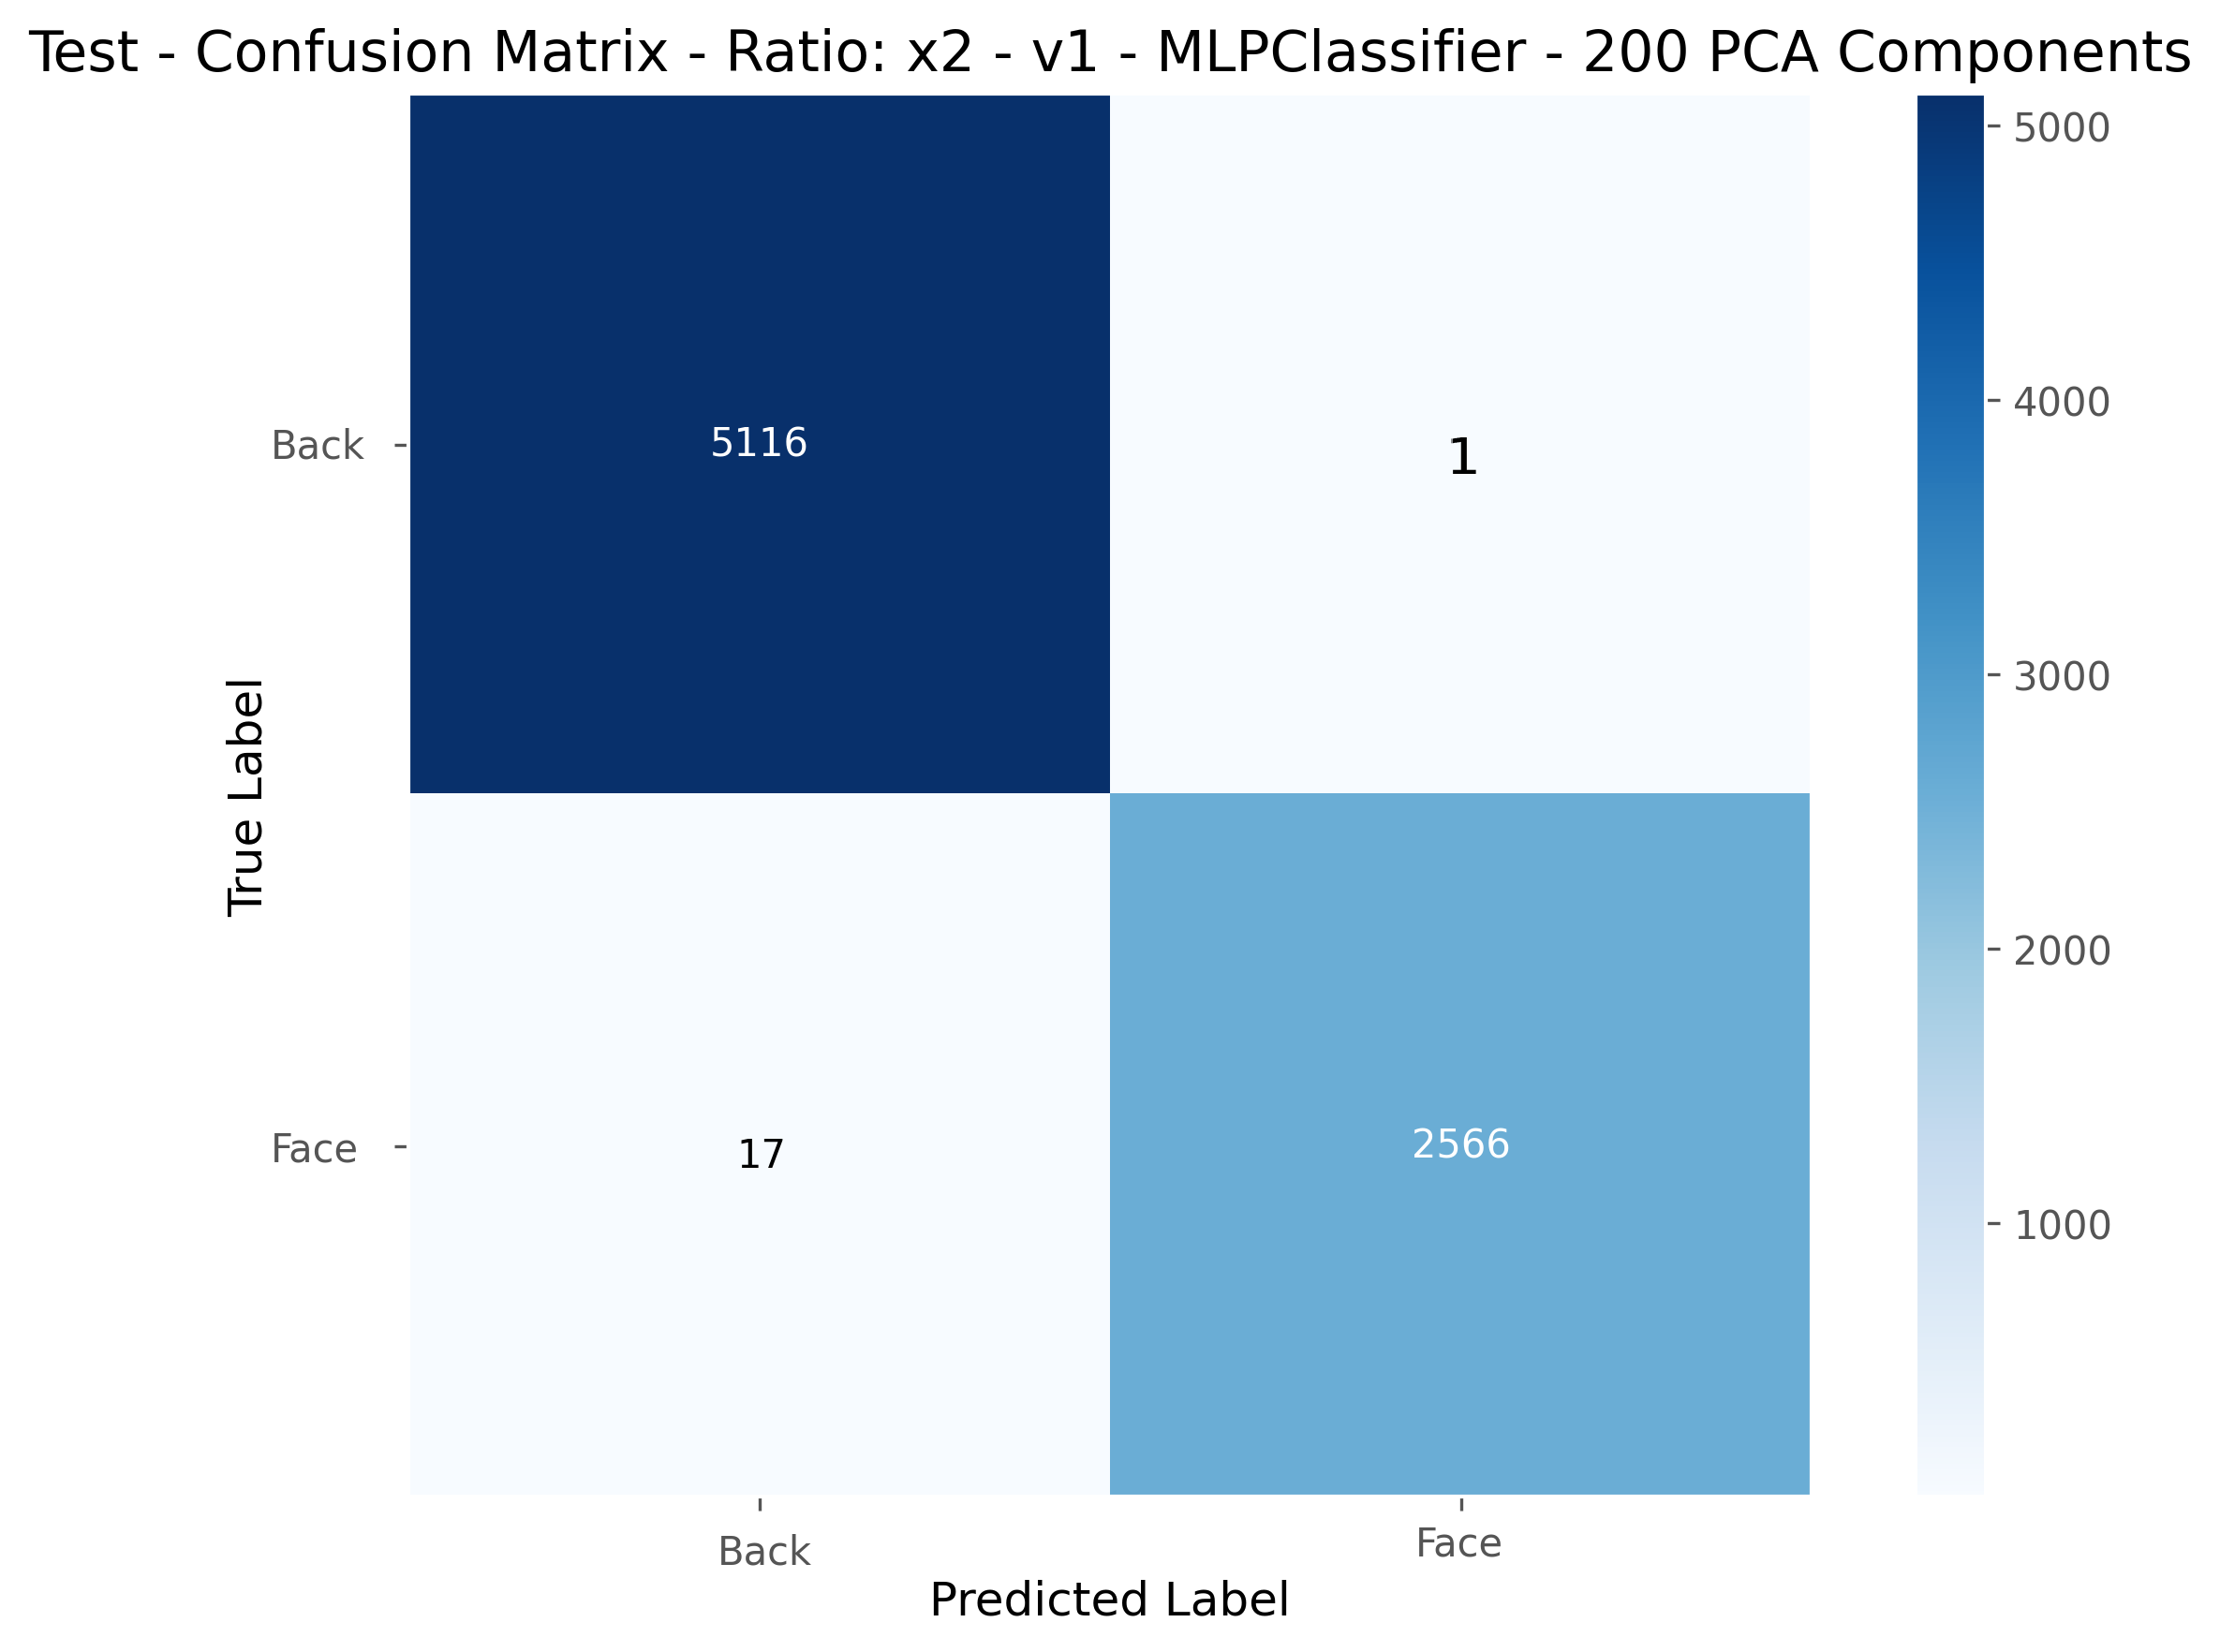
\includegraphics[width=0.7\textwidth]{tarea_5/imagenes/x2_v1_200_MLPClassifier_test_confusion_matrix.png}
    \caption{Matriz de confusión del modelo MLPClassifier con 200 componentes PCA en el conjunto de test.}
    \label{fig:confusion_matrix}
\end{figure}

\begin{figure}[H]
    \centering
    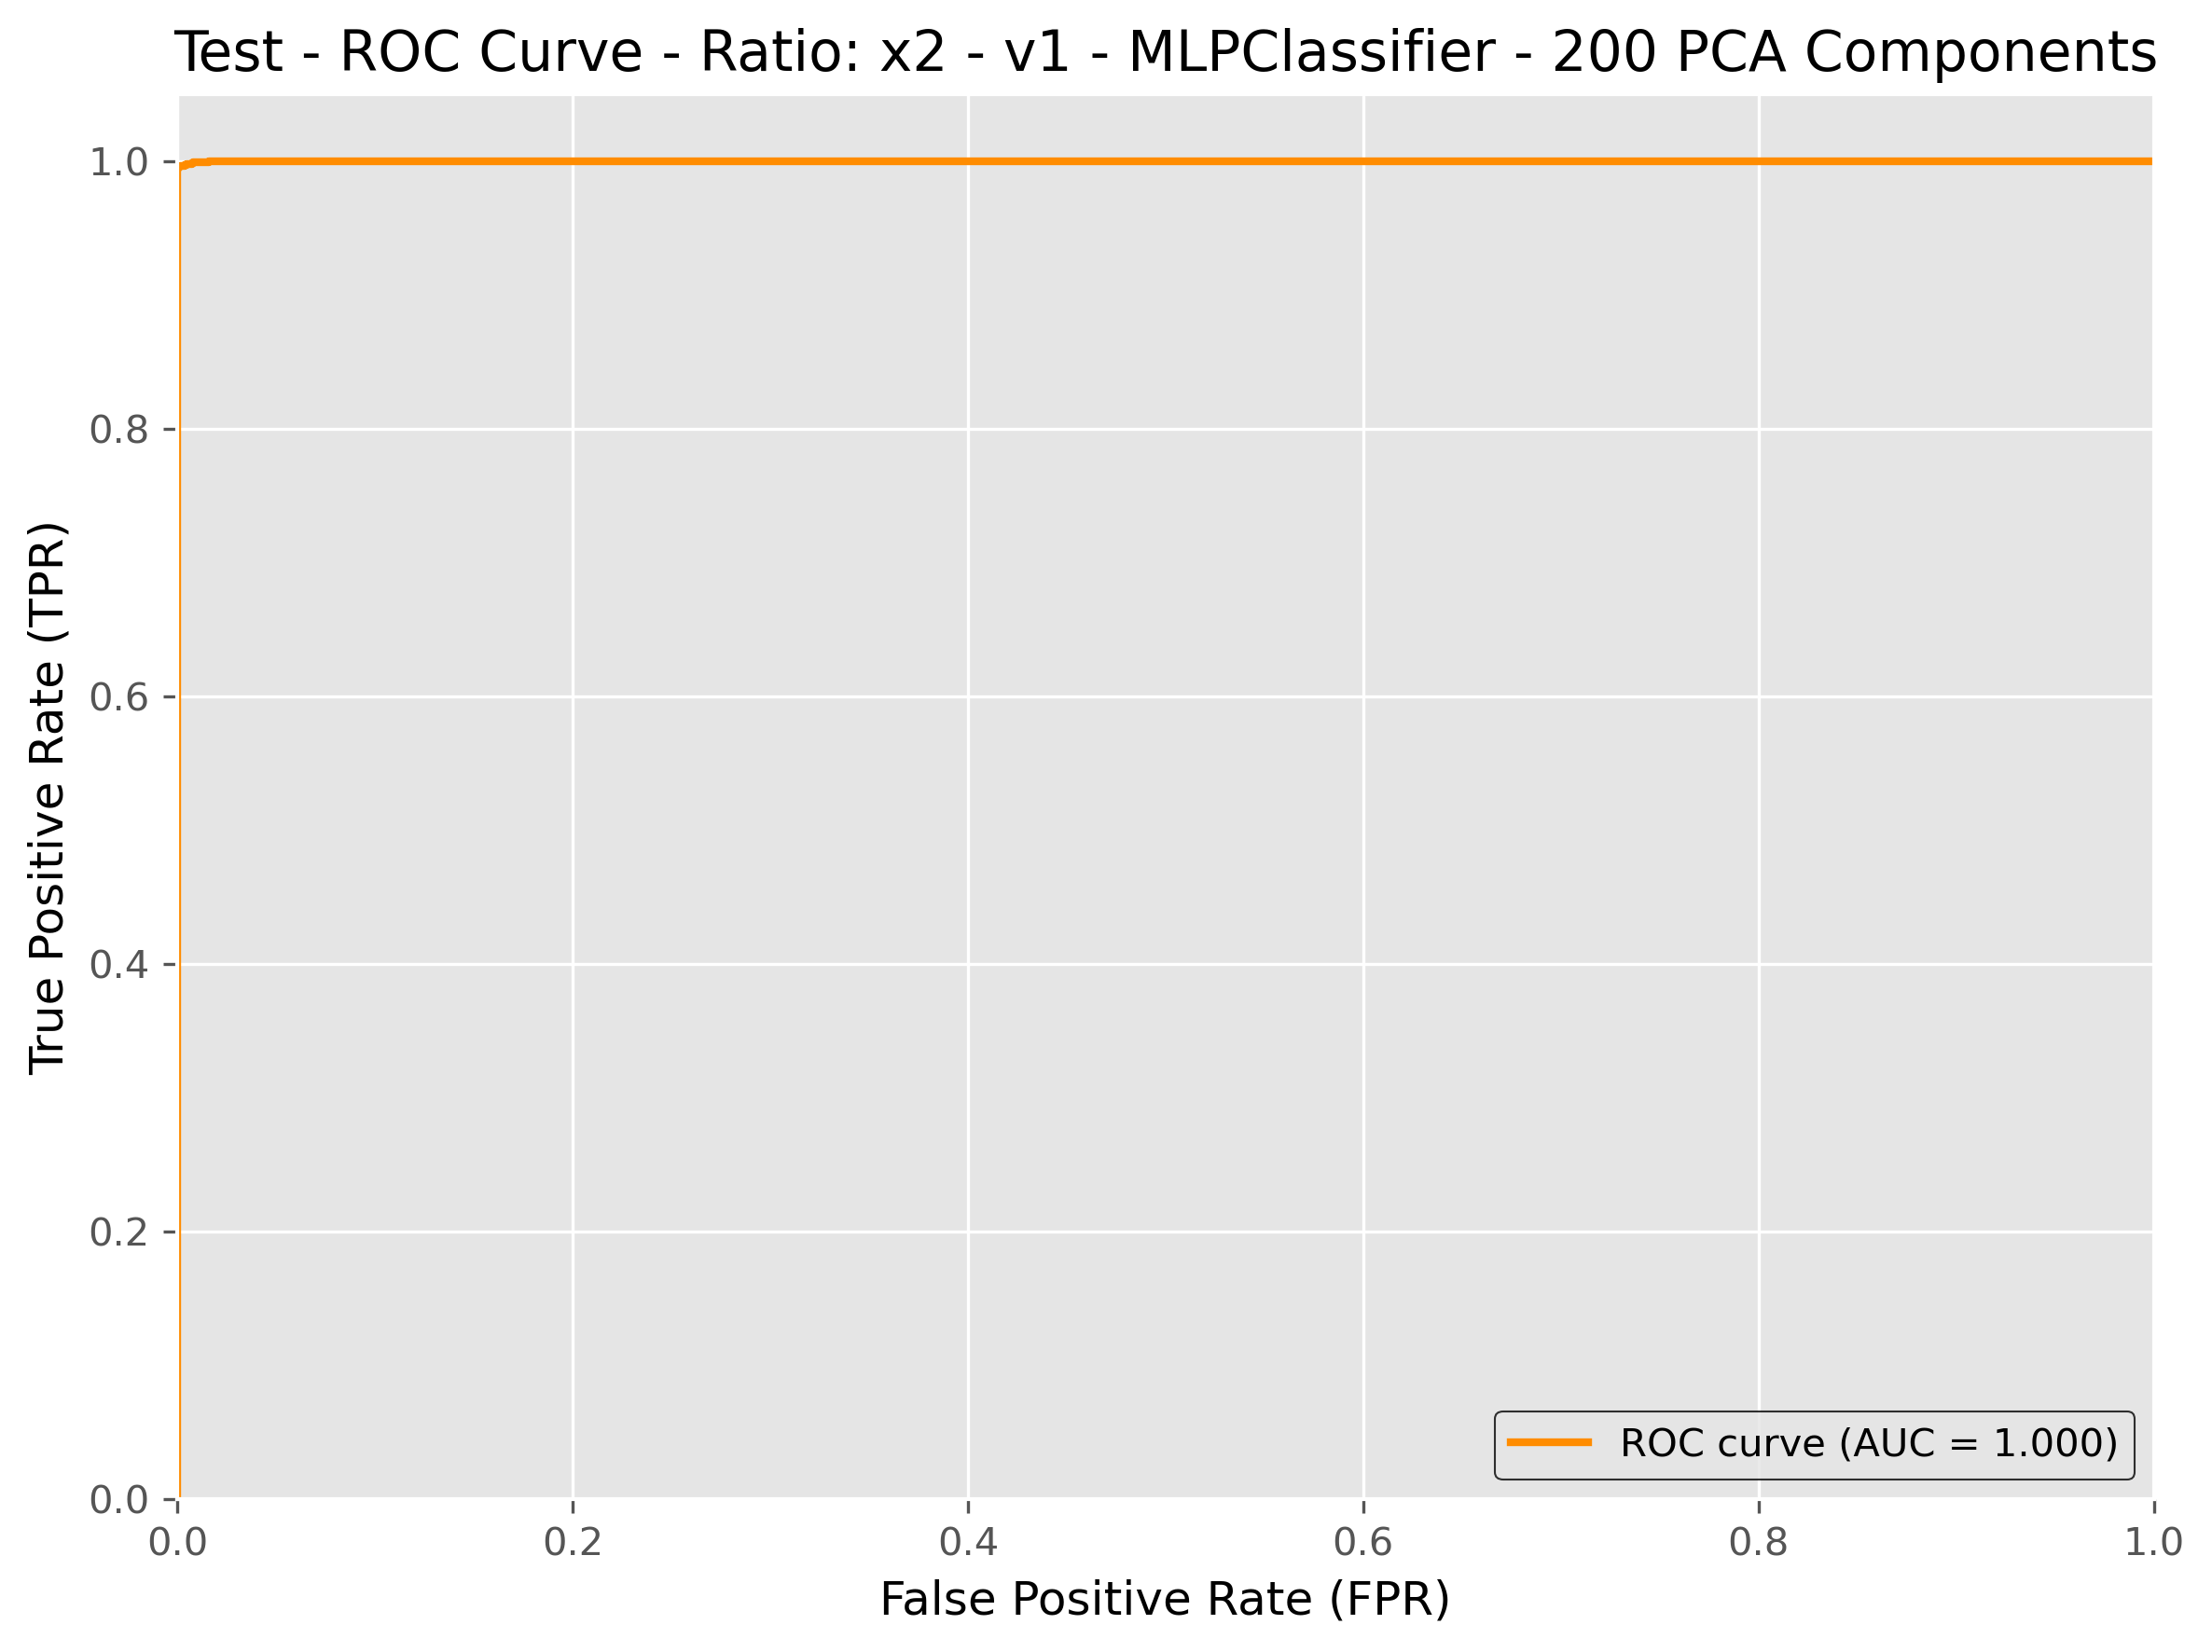
\includegraphics[width=0.7\textwidth]{tarea_5/imagenes/x2_v1_200_MLPClassifier_test_roc_curve.png}
    \caption{Curva ROC del modelo MLPClassifier con 200 componentes PCA en el conjunto de test.}
    \label{fig:roc_curve}
\end{figure}

\textbf{Análisis de resultados}:\\ 

El modelo \textbf{MLPClassifier} con 200 componentes PCA logró el mejor resultado en Kaggle con un F1-Score de 1.00000, demostrando tener una gran capacidad de clasificación de rostros.\\

\textbf{MLPClassifier} mantuvo consistencia entre cross-validation y Kaggle, mientras que \textbf{XGBoost} mostró mejora al entrenar con el dataset completo (F1-Score de 0.98581 a 0.99166). El buen puntaje sugiere que el modelo capturó patrones fundamentales y generalizables de la detección de rostros. El análisis del ranking global revela el buen desempeño del MLPClassifier, ocupando 9 de las 10 mejores posiciones.\\

La metodología de HOG + PCA demostró ser muy efectiva para la detección de rostros. Los descriptores HOG capturaron eficientemente los patrones de gradientes locales característicos de rostros, mientras que PCA con 200 componentes preservó la información discriminativa esencial reduciendo la dimensionalidad y el ruido. Esta configuración preserva aproximadamente el 75\% de la varianza total de las características HOG.\\

\begin{figure}[H]
    \centering
    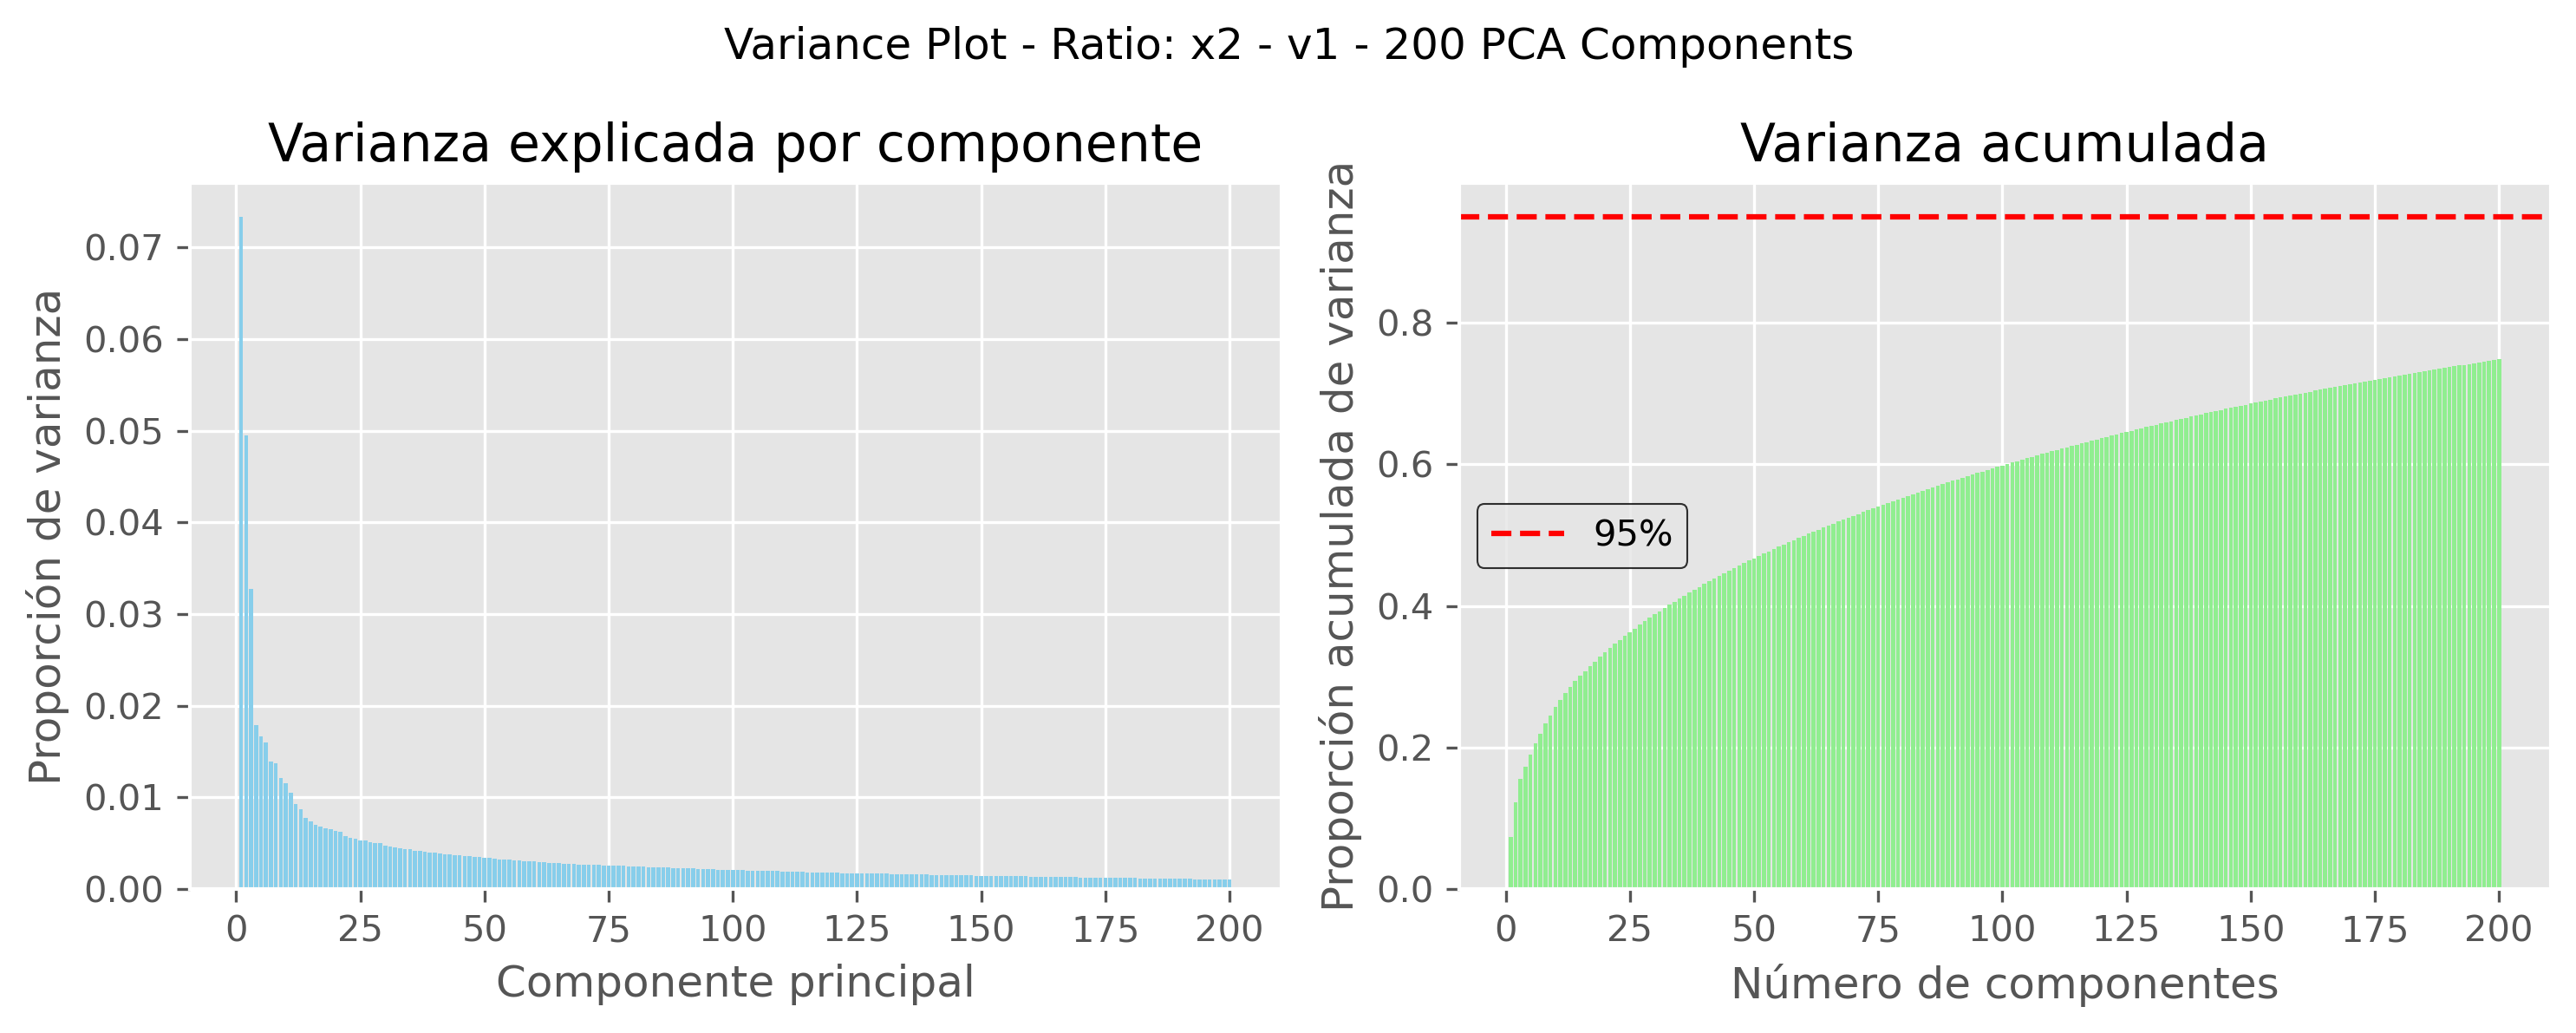
\includegraphics[width=0.8\textwidth]{tarea_5/imagenes/x2_v1_200_PCA_variance_plot.png}
    \caption{Varianza explicada y acumulada por los componentes principales en el modelo MLPClassifier con 200 componentes PCA.}
    \label{fig:pca_variance}
\end{figure}

Por lo tanto, se logró superar la línea base establecida (0.97907) alcanzando 1.00000 en Kaggle, utilizando la combinación HOG + PCA + MLPClassifier.\\

La combinación \textbf{GridSearch + StratifiedShuffleSplit} demostró ser la estrategia más efectiva, logrando el mejor resultado de \textit{f1-score} en cross-validation. Para el modelo MLPClassifier con 200 componentes PCA, esta estrategia alcanzó un \textit{f1-score} para rostros en validación de \textbf{0.9971}, el cual se tradujo en un puntaje perfecto de \textbf{1.00000} en Kaggle. La ventaja de esta estrategia se debe a que combina la exhaustividad de GridSearch con la proporción balanceada de clases (rostros/fondos) en cada división mientras introduce variabilidad aleatoria. De todas formas, todas las estrategias están presentes en los mejores resultados globales. \\

El modelo MLPClassifier final (200 componentes PCA) logró muy buenas métricas:

\begin{table}[H]
    \centering
    \begin{tabular}{|l|c|c|}
    \hline
    \rowcolor{tableblue} \textbf{Métrica} & \textbf{Valor} & \textbf{Interpretación} \\
    \hline
    Accuracy & 0.9977 & 99.77\% clasificaciones correctas \\
    \hline
    Precision & 0.9996 & 99.96\% predicciones positivas correctas \\
    \hline
    Recall & 0.9934 & 99.34\% rostros detectados \\
    \hline
    F1-Score & 0.9965 & Balance óptimo precision/recall \\
    \hline
    AUC-ROC & 0.9999 & Discriminación casi perfecta \\
    \hline
    \end{tabular}
    \caption{Métricas detalladas del modelo final MLPClassifier}
    \label{tab:metricas_finales}
\end{table}

\subsubsection*{Análisis de la Matriz de Confusión}

La matriz de confusión del modelo final (Fig.~\ref{fig:confusion_matrix}) revela un rendimiento excepcional con errores mínimos:

\begin{itemize}
    \item \textbf{Verdaderos Positivos}: 5,116 rostros correctamente clasificados
    \item \textbf{Verdaderos Negativos}: 2,566 fondos correctamente clasificados
    \item \textbf{Falsos Negativos}: Solo 1 rostro no detectado (clasificado como fondo)
    \item \textbf{Falsos Positivos}: 17 fondos clasificados incorrectamente como rostros
\end{itemize}

\subsubsection*{Métricas ROC}

\begin{itemize}
    \item \textbf{TPR (True Positive Rate)}: 0.9934 - Alta capacidad de clasificar rostros reales
    \item \textbf{FPR (False Positive Rate)}: 0.0002 - Tasa extremadamente baja de falsos positivos
    \item \textbf{G-Mean}: 0.9966 - Excelente balance entre TPR y especificidad
\end{itemize}

La curva ROC (Fig.~\ref{fig:roc_curve}) muestra una curva casi ideal, acercándose al punto (0,1) que representa clasificación perfecta.

\pagebreak

\section*{Tarea 6: Detector de Rostros}

\subsection*{Metodología}

El detector sigue un flujo sencillo de cinco pasos:

\begin{enumerate}
    \item \textbf{Pre-procesamiento}  
          Carga la imagen, la convierte a escala de grises, la re-escala a una altura fija (500 px) manteniendo la proporción y verifica que formato y rango sean consistentes con el entrenamiento.

    \item \textbf{Ventana deslizante multiescala}  
          Recorre la imagen con una ventana de 64 × 64 px mientras genera una pirámide de escalas para cubrir rostros grandes y pequeños.

    \item \textbf{Extracción de características}  
          A cada parche se le calcula un descriptor HOG, se normaliza y se reduce su dimensión con PCA, exactamente igual que durante el entrenamiento.

    \item \textbf{Clasificación}  
          El vector resultante se evalúa con el modelo entrenado; sólo se conserva la ventana si su probabilidad de “rostro” supera un umbral configurable.

    \item \textbf{Supresión de no-máximos (NMS)}  
          Las detecciones solapadas se fusionan mediante la métrica IoU, manteniendo la caja con mayor puntuación para obtener un conjunto final único y ordenado.
\end{enumerate}

\subsection*{Optimización de rendimiento}  
Para acelerar el flujo se procesan los parches en \emph{batches} de tamaño \texttt{BATCH\_SIZE} (512) y se reparten en paralelo entre \texttt{MAX\_JOBS} hilos (3). Esta estrategia de procesamiento por lotes y multihilo reduce de forma notable el tiempo total de detección frente a la ejecución secuencial sin afectar la precisión del modelo.

\subsection*{Conjunto de validación}

Para evaluar el detector se utilizó un conjunto de imágenes con rostros, que abarca una variedad de situaciones y condiciones. 

Cada archivo incluye en su nombre el número de rostros presentes, por ejemplo \verb|3-faces_1.jpg| o \verb|10-faces.jpg|.
Esta codificación permite, durante la evaluación, obtener el \emph{ground
truth} directamente a partir del nombre del archivo y calcular de forma
automática las métricas de para cada configuración probada.

\begin{figure}[H]
  \centering
  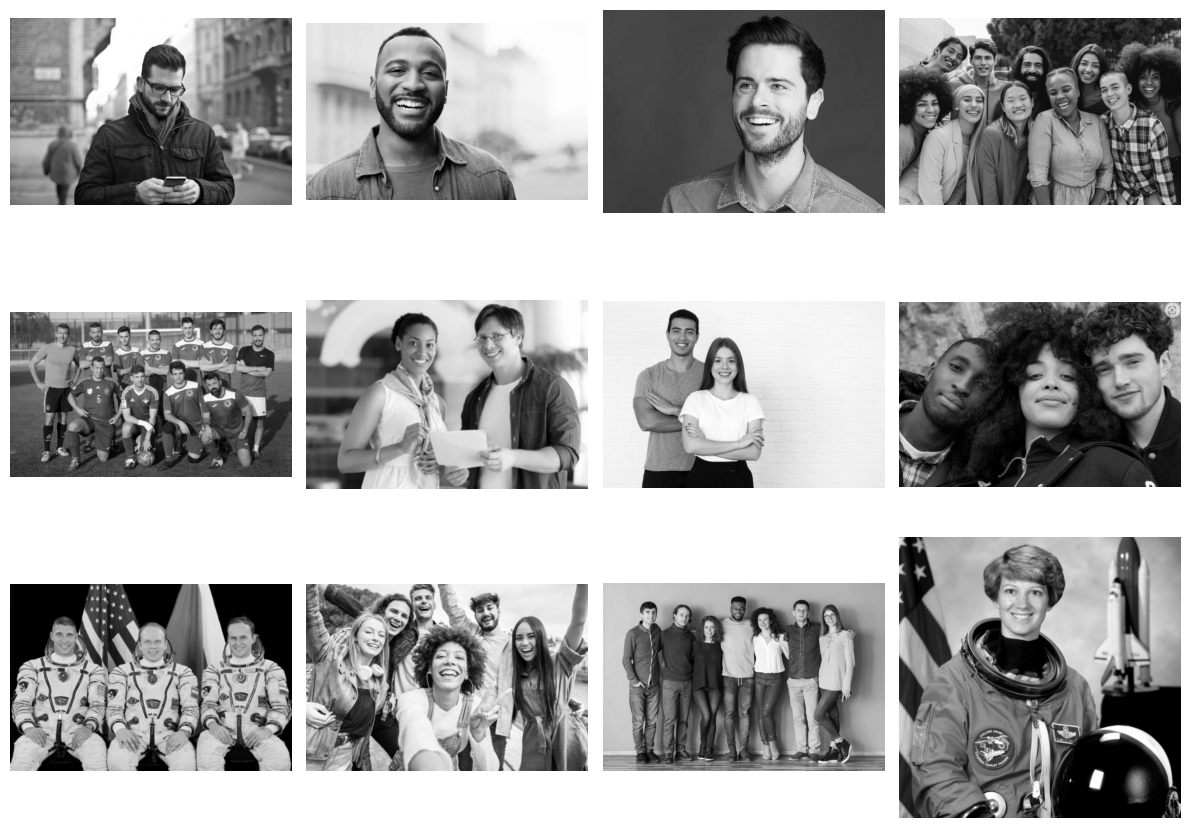
\includegraphics[width=0.65\linewidth]{tarea_6/imagenes/dataset.png}
  \caption{Conjunto de validación.}
  \label{fig:dataset}
\end{figure}

\subsection*{Selección manual de escalas (\texttt{test\_scales})}

Luego de inspeccionar visualmente las imagenes con distintas escalas de recuadros, se adoptó la secuencia
\[
\texttt{test\_scales} = \{\,0.5,\,1.0,\,1.5,\,\dots,\,5.0\}
\]
por las siguientes razones:

\begin{itemize}
    \item \textbf{Cobertura completa}: incluye desde rostros lejanos
          (factor \(0.5{-}1.0\)) hasta primeros planos
          (\(3.5{-}5.0\)).
    \item \textbf{Granularidad equilibrada}: pasos de \(0.5\) evitan
          escalas redundantes y mantienen el tiempo de detección contenido.
    \item \textbf{Consistencia}: con este rango el detector conserva su
          desempeño tanto en fotos de grupo como en retratos de perfil.
\end{itemize}

Con las escalas definidas, se procedió a la búsqueda sistemática de los demás
hiperparámetros.


\subsection*{Búsqueda de hiperparámetros (Grid Search)}
Para afinar el detector se exploraron combinaciones de hiperparámetros clave que afectan su rendimiento. 

\paragraph{Hiperparámetros evaluados}
\begin{itemize}
    \item \textbf{Threshold} (\(\tau\)) — Probabilidad mínima que debe asignar el
          clasificador para que una ventana sea considerada «rostro».
          Umbrales altos favorecen la \emph{precisión} (menos falsos positivos)
          a costa de la \emph{recall}.
    \item \textbf{Step} (\(s\)) — Desplazamiento de la ventana deslizante en
          píxeles.  
          Pasos pequeños exploran más posiciones (mayor recall pero mayor costo
          computacional); pasos grandes aceleran el barrido con riesgo de saltar
          rostros.
    \item \textbf{Overlap} (\(\omega\)) — Umbral de solapamiento
          (\emph{Intersection over Union}) utilizado en la supresión de
          no-máximos. Valores bajos fusionan agresivamente cajas
          superpuestas; valores altos permiten coexistir más recuadros.
\end{itemize}

Los rangos considerados fueron
\(\tau \in \{0.7,\,0.8,\,0.9\}\),
\(s \in \{2,\,4\}\) y
\(\omega \in \{0.05,\,0.20,\,0.30\}\),
lo que generó \(3\times2\times3 = 18\) combinaciones.

\paragraph{Procedimiento}
Para cada una de las \(18\) combinaciones de la rejilla se ejecutó el detector sobre una única imagen de validación: la fotografía del astronauta (\verb|1-astronaut.jpg|).  

Dado que el nombre del archivo codifica el número real de rostros, fue posible
calcular directamente precisión, \emph{recall} y $F_1$-score.  
La Figura~\ref{fig:top5} resume las cinco combinaciones con mejor desempeño.

\begin{figure}[H]
  \centering
  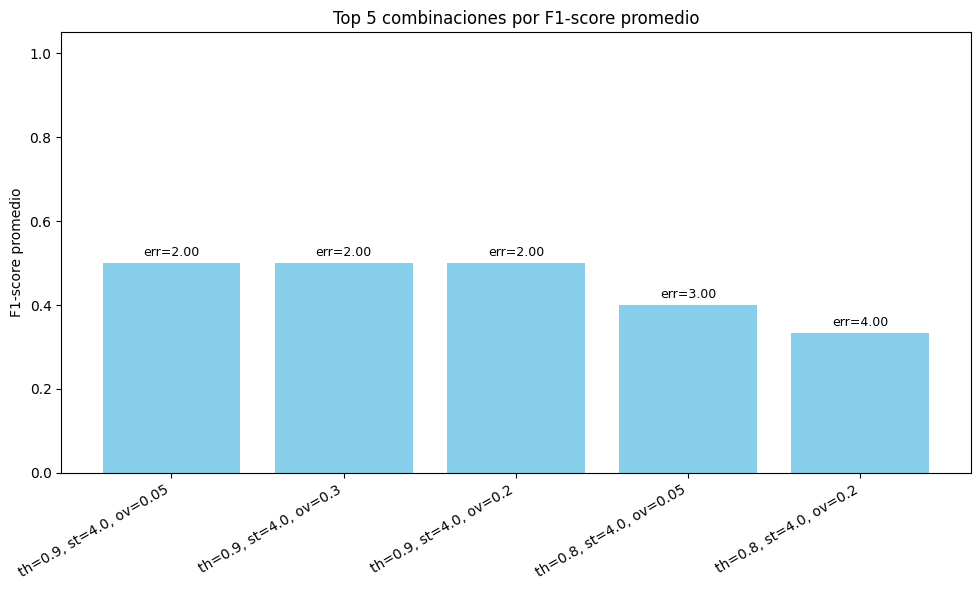
\includegraphics[width=\linewidth]{tarea_6/imagenes/top_combinations_bar.png}
  \caption{Cinco mejores combinaciones ordenadas por $F_1$-score promedio.}
  \label{fig:top5}
\end{figure}

\paragraph{Configuración óptima}
Utilizar \(\tau=0.9\) y \(s=4\) px mejora el equilibrio
precisión/recall, mientras que la supresión con valores de
\(\omega\) entre 0.05 y 0.30 muestra resultados estables.

\subsection*{Pruebas con distintos modelos de clasificación}

Con los hiperparámetros óptimos ya fijados, el siguiente paso fue comprobar qué tan sensibles eran los resultados al modelo de clasificación empleado dentro del detector.

\paragraph{Modelo base (Modelo A)}
Se partió de uno de los clasificadores que mejor se había desempeñado en la
tarea de \emph{clasificación pura}: características HOG cuantizadas en
\(\textbf{50 clases}\) y un \textit{MLPClassifier} entrenado con una relación
\(\text{fondos}:\text{rostros}=2{:}1\).
Al integrarlo en el pipeline completo se observó un número elevado de falsos
positivos, indicando que el modelo no era lo bastante estricto al distinguir
entre rostro y fondo.

\paragraph{Ajuste del balance de clases}
Para reducir esos falsos positivos se ensayaron dos variantes en las que se
incrementó progresivamente la proporción de ejemplos de fondo durante el
entrenamiento:

\begin{center}
\begin{tabular}{ll}
\textbf{Modelo B} & Ratio fondos:rostros = 12:1 \\[2pt]
\textbf{Modelo C} & Ratio fondos:rostros = 24:1
\end{tabular}
\end{center}

\subsection*{Resultados}
Las Figuras~\ref{fig:modelos-1f}–\ref{fig:modelos-10f} ilustran, para varias
imágenes de prueba, cómo se comporta cada modelo (recuadros azules indican las
ventanas obtenidas tras NMS):

\begin{itemize}
    \item \textbf{Modelo A} presenta numerosos falsos positivos, sobre todo en
          texturas de fondo o partes del cuerpo con bordes pronunciados.
    \item \textbf{Modelo B} reduce parcialmente los falsos positivos, pero aún
          genera recuadros espúreos y sobredimensionados en escenas complejas.
    \item \textbf{Modelo C} conserva las detecciones correctas y elimina casi
          por completo los falsos positivos, incluso en imágenes con muchos
          rostros (6–10 personas), confirmando la intuición de que un mayor
          sesgo hacia la clase «fondo» fortalece la discriminación.
\end{itemize}

\paragraph{Conclusión} 
El \textbf{Modelo C} (ratio 24:1) demostró el mejor equilibrio entre
\emph{recall} y precisión visual, por lo que se adoptó como clasificador final
del detector.

\begin{figure}[H]
  \centering
  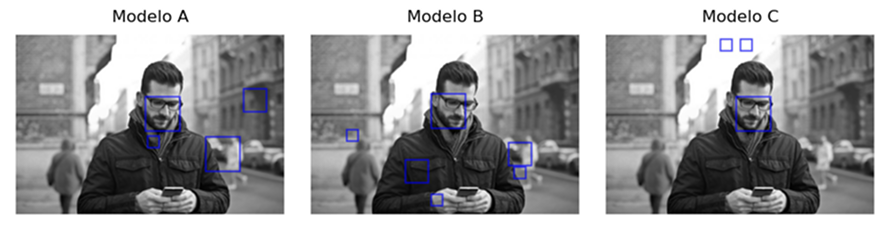
\includegraphics[width=\linewidth]{tarea_6/imagenes/1-faces_1.png}\\[4pt]
  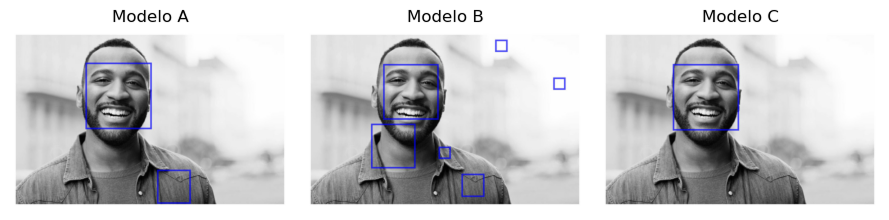
\includegraphics[width=\linewidth]{tarea_6/imagenes/1-faces_2.png}\\[4pt]
  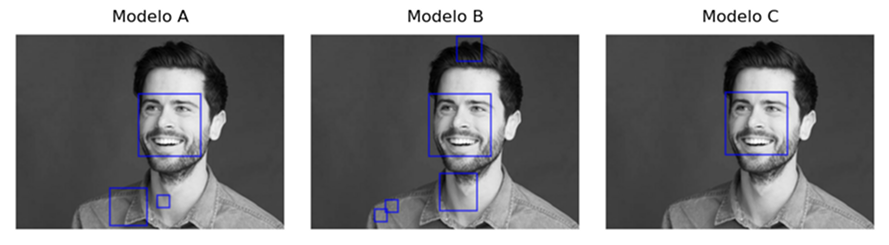
\includegraphics[width=\linewidth]{tarea_6/imagenes/1-faces_3.png}
  \caption{Ejemplos con una cara: comparación de los tres modelos.}
  \label{fig:modelos-1f}
\end{figure}

\begin{figure}[H]
  \centering
  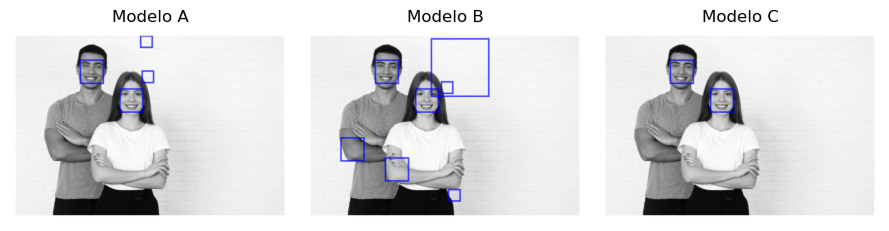
\includegraphics[width=\linewidth]{tarea_6/imagenes/2-faces_2.png}
  \caption{Ejemplo con dos caras: reducción progresiva de falsos positivos.}
  \label{fig:modelos-2f}
\end{figure}

\begin{figure}[H]
  \centering
  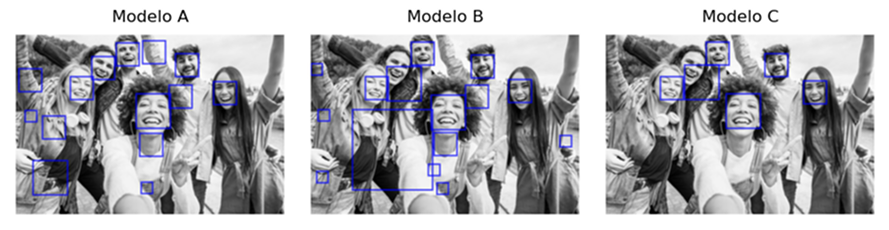
\includegraphics[width=\linewidth]{tarea_6/imagenes/6-faces.png}\\[4pt]
  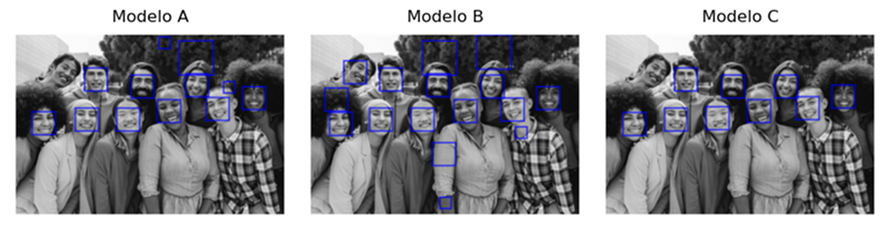
\includegraphics[width=\linewidth]{tarea_6/imagenes/10-faces.png}
  \caption{Escenas con múltiples rostros: el Modelo C mantiene detecciones limpias.}
  \label{fig:modelos-10f}
\end{figure}

En síntesis, aumentar el ratio de fondos a rostros durante el entrenamiento del clasificador resultó decisivo para lograr un equilibrio convincente entre las detecciones correctas y los falsos positivos.


\pagebreak

\appendix

\section*{Código Fuente}
% Referencia al repositorio o archivos de código
% Link al repositorio: \url{https://github.com/usuario/repositorio}

\end{document}
